%%%%%%%%%%%%%%%%%%%%%%% file template.tex %%%%%%%%%%%%%%%%%%%%%%%%%
%
% This is a general template file for the LaTeX package SVJour3
% for Springer journals.          Springer Heidelberg 2010/09/16
%
% Copy it to a new file with a new name and use it as the basis
% for your article. Delete % signs as needed.
%
% This template includes a few options for different layouts and
% content for various journals. Please consult a previous issue of
% your journal as needed.
%
%%%%%%%%%%%%%%%%%%%%%%%%%%%%%%%%%%%%%%%%%%%%%%%%%%%%%%%%%%%%%%%%%%%
%
% First comes an example EPS file -- just ignore it and
% proceed on the \documentclass line
% your LaTeX will extract the file if required
\begin{filecontents*}{example.eps}
%!PS-Adobe-3.0 EPSF-3.0
%%BoundingBox: 19 19 221 221
%%CreationDate: Mon Sep 29 1997
%%Creator: programmed by hand (JK)
%%EndComments
gsave
newpath
  20 20 moveto
  20 220 lineto
  220 220 lineto
  220 20 lineto
closepath
2 setlinewidth
gsave
  .4 setgray fill
grestore
stroke
grestore
\end{filecontents*}
%
\RequirePackage{fix-cm}
%
%\documentclass{svjour3}                     % onecolumn (standard format)
%\documentclass[smallcondensed]{svjour3}     % onecolumn (ditto)
\documentclass[smallextended]{svjour3}       % onecolumn (second format)
%\documentclass[twocolumn]{svjour3}          % twocolumn
%
\smartqed  % flush right qed marks, e.g. at end of proof
%
\usepackage{graphicx}
%
% \usepackage{mathptmx}      % use Times fonts if available on your TeX system
%
% insert here the call for the packages your document requires
%\usepackage{latexsym}
% etc.
%
% please place your own definitions here and don't use \def but
% \newcommand{}{}
%
% Insert the name of "your journal" with
% \journalname{myjournal}
%


\usepackage{color}
\usepackage{amsfonts,amsmath,algorithm,graphicx,subfigure}
\usepackage{booktabs} 
\usepackage[noend]{algorithmic}

\newcommand{\la}{\ell}



\begin{document}

\title{A Faster Algorithm for Cuckoo Insertion and Bipartite Matching in Large Graphs%\thanks{Grants or other notes
%about the article that should go on the front page should be
%placed here. General acknowledgments should be placed at the end of the article.}
}
%\subtitle{Do you have a subtitle?\\ If so, write it here}

%\titlerunning{Short form of title}        % if too long for running head

\author{Avishek Anand        \and
        Megha Khosla %etc.
}

%\authorrunning{Short form of author list} % if too long for running head

\institute{F. Author \at
              first address \\
              Tel.: +123-45-678910\\
              Fax: +123-45-678910\\
              \email{fauthor@example.com}           %  \\
%             \emph{Present address:} of F. Author  %  if needed
           \and
           S. Author \at
              second address
}

\date{Received: date / Accepted: date}
% The correct dates will be entered by the editor

%\documentclass[a4paper,11pt]{article}
%\usepackage{a4wide}
%\usepackage{color}
%\usepackage{amsfonts,amsmath,amsthm,algorithmic,algorithm, graphicx,subfigure}
%%\usepackage[usenames]{color}
%%\usepackage[notref,notcite]{showkeys}
%%\usepackage[dvips]{graphicx}
%
%\def\noproof{{\unskip\nobreak\hfill\penalty50\hskip2em\hbox{}\nobreak\hfill%
%       $\square$\parfillskip=0pt\finalhyphendemerits=0\par}\goodbreak}
%
%
\newcommand{\eps}{\varepsilon}
\newcommand{\al}{\alpha}
\newcommand{\be}{\beta}
\newcommand{\Nat}{\mathbb{N}}
\newcommand{\prob}{\mathbb{P}}
\newcommand{\ex}{\mathbb{E}}
\newcommand{\Pa}{{\mathcal P}}
\newcommand{\U}{{\mathcal U}}
\newcommand{\B}{{\mathcal B}}
\newcommand{\es}{{\mathcal S}}
\newcommand{\E}{{\mathbb E}}
\newcommand{\W}{{\mathcal W}}
\newcommand{\F}{{\mathcal F}}
\newcommand{\M}{{\mathcal M}}
\newcommand{\C}{{\textsc C}}
\newcommand{\D}{{\mathcal D}}
\newcommand{\X}{{\mathcal X}}
\newcommand{\Q}{{\mathcal Q}}
\newcommand{\A}{{\mathcal A}}
\newcommand{\La}{{\mathcal L}}
\newcommand{\T}{{\mathcal T}}
\newcommand{\G}{{\mathcal{G}}}
\newcommand{\ga}{\gamma}
\newcommand{\Bin}{\mathrm{Bin}}
\newcommand{\Aux}{{\mathcal G}}
\newcommand{\Li}{{\mathcal L}}
\newcommand{\N}{{\mathcal N}}
\newcommand{\I}{{\mathcal I}}
\newcommand{\It}{\tilde{\mathcal I}}
\newcommand{\Is}{\tilde{I}}
\newcommand{\Nt}{\mathcal N}
\newcommand{\nt}{\tilde{N}}
\newcommand{\Ub}{\overline{U}}
\newcommand{\Hi}{\mathcal H}
\newcommand{\va}{\overline{a}}
\newcommand{\Exx}{\mathrm{Ex}}
\newcommand{\Pl}{\mathsf{P}}
\newcommand{\Nl}{\mathsf{N}}
\newcommand{\Cl}{\mathsf{C}}
\newcommand{\Bl}{\mathsf{B}}



\newcommand{\Y}{{\mathcal{Y}}}
\newcommand{\BP}{{\mathbb{P}}}

\newcommand{\MN}{{\mathcal{N}}}
\newcommand{\CN}{{\mathcal{N}}}
\newcommand{\CS}{{\mathcal{S}}}
\newcommand{\CE}{{\mathcal{E}}}
\newcommand{\CP}{{\mathcal{P}}}
\newcommand{\CH}{{\mathcal{H}}}
\newcommand{\CT}{{\mathcal{T}}}
\newcommand{\Net}{{\mathtt{Net}}}
\newcommand{\Ber}{{\mathtt{Be}}}
\newcommand{\Be}{{\mathtt{Be}}}
\newcommand{\Ser}{{\mathtt{Ser}}}
\newcommand{\Par}{{\mathtt{Par}}}
\newcommand{\sh}{{\mathtt{sh}}}
\newcommand{\Set}{{\mathsf{Set}}}

\renewcommand{\Pr}[1]{\mathbb{P}\left(#1\right)}




\newcommand{\keyword}[1]{\textbf{#1}~}
%\newcommand{\IF}{\keyword{if}}
%\newcommand{\ELSEIF}{\keyword{ELSEIF} }
%\newcommand{\THEN}{\keyword{then} }
%\newcommand{\ELSE}{\keyword{else}}
%\newcommand{\RETURN}{\keyword{return}}
%\newcommand{\FOR}{\keyword{for}}
%\newcommand{\FOREACH}{\keyword{foreach}}
%\newcommand{\DO}{\keyword{DO} }
%\newcommand{\AND}{\keyword{AND} }
%\newcommand{\OR}{\keyword{OR} }
\newcommand{\Pcl}{\widetilde{H}_{n,p,k}}


%
%\numberwithin{equation}{section}
%\numberwithin{firsttheorem}{section}
%\title{\centering{Linear Time algorithm for Cuckoo Insertion}}
%\date{}
%\author{Megha Khosla}
%\begin{document}
%
\maketitle
\abstract{Hash tables are ubiquitous in computer science for their use in storing large sets of data. Cuckoo hashing is an efficient technique of creating large hash tables with high space utilization and offers a guaranteed constant access time. We are given $n$ locations and $m$ items. Each item has to be placed in one of the $k\ge2$ locations chosen by $k$ random hash functions. By allowing more than one choice for a single item, cuckoo hashing resembles multiple choice allocations schemes. In addition it supports dynamically changing the location of an item among its possible locations. We propose and analyze an insertion algorithm for cuckoo hashing that runs in \emph{linear time} with high probability and in expectation. Previous work on total allocation time has analysed breadth first search, and it was shown  to be linear only in \emph{expectation}. Our algorithm finds an assignment (with probability 1) whenever it exists. In contrast, the other known insertion method also called  \emph{random walk insertion} may run indefinitely even for a solvable instance.
We present experimental results comparing the performance of our algorithm with the random walk method. 

As a corollary we obtain a linear time algorithm(with high probability and in expectation) for finding perfect matchings in a special class of sparse random bipartite graphs. We also perform experiments for finding maximum matchings in general large bipartite graphs and report an order of magnitude improvement in the running time as compared to Hopkraft Karp matching algorithm.
} 

\section{Introduction}
In computer science, hash table~\cite{bookC:09} is a data structure that maps items (keys) to locations (values) using a hash function. More precisely, given a universe $U$ of items and a hash table $H$ of size $n \in \mathbb{N}$, a hash function
$h : U \rightarrow \{1,2,\ldots, n\}$ maps the items from $U$ to the $n$ positions on the table. Ideally, the hash function should assign to each possible item to a unique location, but this ideal is rarely achievable in practice. Two or more items could be mapped to the same location resulting in a collision. In this work we deal with a collision resolution technique known as \emph{cuckoo hashing}.  Cuckoo hashing was first proposed by Pagh and Rodler in \cite{inp:pr01}. We are interested in a generalization of the original idea (see~\cite{inc:fpss03}) where we are given a table with $n$ locations, and we assume each location can hold a single item. Each item chooses randomly $k\ge 3$ locations (using $k$ random hash functions) and has to be placed in one of them.  Formally speaking we are given $k\ge3$ hash functions $h_1, . . . , h_k$
that each maps an element $x \in U$ to a position in the table $H$. 
Moreover we assume that $h_1, . . . , h_k$ are truly independent and random hash functions. We refer the reader to ~\cite{ms:08,d:09}  (and references therein) for justification of this idealized assumption. 
 Other variations of cuckoo hashing are considered in for example \cite{inp:ans:09,art:kmw09}.

%Multiple choice load balancing can be abstracted as a balls-into-bin game. In this scenario we are given $n$ bins (locations, servers) and  $m=\lfloor cn\rfloor$ balls (items, users, tasks) where each ball chooses $k$ bins randomly and is placed into one of them. A first breakthrough was achieved by~\cite{art:abku99} where the authors consider the case $c=1$ and $k=2$. 
%They show that if each ball is placed into the one which is least loaded at the time of placement then with high probability the maximum load is ${\log \log n \over \log 2} +O(1).$ This is an exponential improvement compared to the case where $k=1$, i.e., ball is placed into one of the random bins. Since then a large amount of literature has appeared considering load balancing schemes for $k\ge2$. Most of the schemes never change the location of a ball once it is placed. Our algorithm, in addition, combines the power of multiple choices with the power of dynamically changing the location of balls among its $k$ chosen bins. Our algorithm finds applications in the following scenarios.

Cuckoo hashing resembles multiple choice allocations schemes in the sense that it allows more than one choice for a single item. In addition it supports dynamically changing the location of an item among its possible locations during insertion. The insertion procedure in cuckoo hashing goes as follows. Assume that $p$ items have been inserted, each of them having made their $k$ random choices on the hash table, and we are about to insert the $p+1$st item. This item selects its $k$ random locations from the hash table and is assigned to one of them. But this location might already be occupied by a previously inserted item. In that case, the previous item is kicked out and is assigned to one of the other $k-1$ selected locations. In turn, this position might be occupied by another item, which is kicked out and goes to one of the remaining $k-1$ chosen locations. This process may be repeated indefinitely or until a free loction is found. 

We model cuckoo hashing by a directed graph $G=(V,E)$  such that the set of vertices $V=\{v_1,v_2,\ldots,v_n\}$ corresponds to locations on the hash table. We say a vertex is \emph{occupied} if there is an item assigned to the corresponding location, otherwise it is \emph{free}. Let $\mathcal{I}$ be the set of $m$ items. We represent each item $x\in\mathcal{I} $ as a tuple of its $k$ chosen vertices (locations), for example, $x=(v_{x_1},v_{x_2},\ldots , v_{x_k})$.
A directed edge $e=(v_i,v_j) \in E$ if and only if there exists an item $y\in \mathcal{I} $ so that the following two conditions hold, (i) $v_i,v_j \in y$, and (ii) $v_i$ is occupied by $y$. Note that a vertex with outdegree $0$ is a free vertex. We denote the set of free vertices by $F$ and the distance of any vertex $v$ from some vertex in $F$ by $d(v,F)$. Since $G$ represents an allocation we call $G$ an \emph{allocation graph}. 

%AWe then repeat the procedure for the replaced item. We say an \emph{assignment} is made whenever an item is placed on a chosen vertex.We repeat the above procedure for the kicked out item. 

Now assume that in the cuckoo insertion procedure, at some instance an item $z$ arrives such that all its $k$ choices are occupied. Let $v_j\in z$ be the vertex chosen to place item $z$. The following are the main observations.

 \begin{enumerate}
\item The necessary condition for item $z$ to be successfully inserted at $v_{z_j}$ is the existence of a path from $v_{z_j}$ to $F$. This condition remains satisfied as long as some allocation is possible.
\item The procedure will stop in the minimum number of steps if for all $v_{z_i}\in z$  the distance $d(v_{z_j},F)\le d(v_{z_i},F)$. \end{enumerate}

With respect to our first observation, a natural question would be the following. We are given a set of $m$ items and $n$ locations such that each item picks $k\ge 3$ locations at random. Is it possible to place each of the items into one of their chosen locations such that each location holds at most one item? From~ \cite{inp:l12, fp12,fm12} we know that there exists a critical size $c_k^* n$ such that if $m<c_k^* n$ then such an allocation is possible with high probability, otherwise this is not the case.


\begin{theorem}
\label{thm:mainO}
For integers~$k\geq 3$ let~$\xi^\ast$ be the unique solution of the equation
\begin{equation}\label{eq:kxi}
 k = {\xi(1-e^{-\xi})\over 1-e^{-\xi} -\xi e^{-\xi} }.
\end{equation}
Let~$c_{k}^\ast= \frac{\xi^\ast}{k(1-e^{-\xi^{*}})^{k-1}}$. Then
\begin{equation}
\label{eq:phnmkl}
	\Pr{\text{allocation of $m=\lfloor cn\rfloor$ items to $n$ locations is possible}}
	\stackrel{(n \to \infty)}{=} 
	\begin{cases}
		0, & \text{ if } c > c_{k}^\ast \\
		1, & \text{ if } c < c_{k}^\ast
	\end{cases}.
\end{equation}
\end{theorem}

The proof of the above theorem is non-constructive, i.e., it does not give us an algorithm to find such an allocation. In this work we deal with the algorithmic issues and propose an algorithm which takes linear time with high probability to find the optimal allocation.

Our second observation suggests that the insertion time in the cuckoo hashing depends on the selection of the location, which we make for each assignment, from among the $k$ possible locations. One can in principle use breadth first search to  always make assignments over the shortest path (in the allocation graph). But this method is inefficient and expensive to perform for each item. One can also select uniformly at random a location from the available locations. This resembles a random walk on the locations of the table and is called the \emph{random walk insertion}. In~\cite{art:fps10,art:fmm11} the authors analyzed the random walk insertion method and gave a polylogarithmic bound (with high probability) on the maximum insertion time, i.e., the maximum time it can take to insert a single item.  



\subsection{More on Related Work}
The allocation problem in cuckoo hashing can also be phrased in terms of \emph{orientation of graphs} or more generally \emph{orientations of $k$-uniform hypergraphs}. The $n$ locations are represented as vertices and each of the $m$ items form an edge with its $k$-vertices representing the $k$ random choices of the item.
In fact, this is a random (multi)hypergraph $H^*_{n,m,k}$ (or random (multi)graph $G^*_{n,m}$ for $k=2$) with $n$ vertices and $m$ edges where each edge is drawn uniformly at random ( with replacement) from the set of all $k$-multisubsets of the vertex set. An $\la$-orientation of a graph then amounts to a mapping of each edge to one of its vertices such that no vertex receives more than $\la$ edges. $\la$ is also called the maximum load capacity. In our algorithm, we focus on $\la=1$. Here, we give an overview of existing work for general $\la$ for completeness.

For the case $k = 2$, several allocation algorithms and their analysis are closely connected to the cores of the associated
graph. The $\la$ core of a graph is the maximum vertex induced subgraph with minimum degree at least $\la$. 
For example, Czumaj and Stemann~\cite{ina:cs01} gave a linear time algorithm achieving maximum load $O(m/n)$ based on computation of all cores. The main idea was to repeatedly choose a
vertex $v$ with minimum degree and remove it from the
graph, and assigning all its incident edges (balls) to vertex (bin) $v$. 

Cain, Sanders, and Wormald~\cite{1283433}  used a variation of the above approach and gave a linear time algorithm for computing an optimal allocation (asymptotically almost surely). Their algorithm first guesses the optimal load among the two likely values values ($\lceil m/n\rceil $ or $\lceil m/n\rceil +1$). The algorithm starts with load value say $\la=\lceil m/n\rceil $. Each time a vertex with degree at most $\la$ and its incident edges are assigned to $v$. The above rule also called the mindegree rule will first reduce the graph to its $\la+1$ core. After that some edge $(u,v)$ is picked according to some priority rule and assigned to one of its vertices. Again the mindegree rule is applied with respect to some conditions. In case the algorithm fails it is repeated after incrementing the load value.

Fernholz and Ramachandran~\cite{1283432} used a different approach of dealing with the vertices with degree greater than the maximum load.  Their algorithm also called \emph{excess degree reduction} (EDR) always chooses a vertex with minimum degree, $d$. If $d<\la$ then this vertex is assigned all its incident edges and is removed from the graph. In case $d>2\la$ the algorithm fails. Otherwise, EDR replaces $d-\la$ paths of the form
$(u, v, w)$ by bypass edges $(u, w)$ and then orients all remaining edges ($\le \la$ ) incident to $v$
towards $v$.

%Note that the above described algorithms requires the complete knowledge of the graph right from the beginning. In contrast we might need methods to assign items in an online manner, i.e., items make their random choices only on arrival and have to be assigned as and when they arrive. Such methods usually involve moving of balls among its chosen locations whenever required. For example, in cuckoo hashing, when an item $i$ appears it is assigned to one of its free choices. In case all its $k$ choices are occupied, then one of its chosen locations say $loc$ is selected. One of the items already placed on $loc$ is moved out and the item $i$ is placed. The moved out item then looks for a free location among its other choices and the procedure is repeated till an empty location is found. 
%
%It is often useful to understand cuckoo hashing in a graph theoretic setting, where each item corresponds to a vertex on one side of a bipartite graph and locations correspond to vertices on the other side. There is an edge between each item and its chosen locations. Then the sequence of moves for assigning an item (described in the previous paragraph) defines an augmenting path in this graph. 
%
%For the online setting, the case $k=2$ and $\la=1$ is well understood~\cite{inp:pr01, Devroye2003215}. Note that for each move (except the first one) there is exactly one choice for the algorithm. The case $k\ge 3$ is more interesting. For $k=3$ and $\la=1$, Fotakis et. al ~\cite{inc:fpss03} provides a \emph{breadth first search} (BFS) approach. Essentially, if the  $k$ choices for the item $i$ are full, one considers the other choices of the $k$
%items in those locations, and if all those locations are filled, one considers the other choices of the
%items in those locations, and so on. The total allocation time with this approach is shown to be linear only in expectation.
%
%For the same case,  Frieze, Melsted and Mitzemmacher~\cite{fm12}, and Fountoulakis, Panagiotou and Steger~\cite{art:fps10} analyzed the \emph{random walk method}, in which one chooses a location randomly from among the $k$ filled choices of an item. More precisely if the $k$ choices of an item $i$ are full, one chooses a random location, say $loc$ from among the $k$ locations. The already placed item, say $i'$ is moved out to make room for $i$. The item $i'$ then looks for an empty location from among its $k-1$ choices. If all its choices are full a location is again selected randomly and the above procedure is repeated. Both of the above mentioned works gave polylogarithmic bounds for maximum allocation time.

%Their analysis also determined the threshold for $s$-orientability of sparse random graphs which is also the threshold for the $s+1$ core to have density (ratio of number of edges to that of vertices) less than $s$. 
\noindent Optimal allocations can also
be computed in polynomial time using maximum 
flow computations and with high probability achieve a maximum load of 
$\lceil m/n\rceil$ or $\lceil m/n\rceil +1$~\cite{sek99}. 

\paragraph{Notations.} Throughout the paper we use the following notations. We denote the set of integers $\{1,2,\ldots, n\}$ by $[n]$. Let $V=\{v_1,v_2,\ldots, v_n\}$ be the set of $n$ vertices representing the locations of the hash table. For an allocation graph $G=(V,E)$ and any two vertices $v_i,v_j\in V$, the shortest distance between $v_i$ and $v_j$ is denoted by $d(v_i,v_j).$  We denote the set of free vertices by $F$. We denote the shortest distance of a vertex $v_i\in V$ to any set of vertices say $S$ by $d(v_i,S)$ which is defined as \[d(v_i,S): = \min_{v_j\in S} d(v_i,v_j).\] We use $R$ to denote the set of vertices furthest from $F$, i.e.,
\[   R:= \{ v_i\in V |d(v_i, F ) \ge \max_{ v_j \in V} d(v_j,F)\}.
\]
For some integer $t\in[n]$ and the subset of vertex set $V' \subset V$ let ~$N_{t}(v_i)$ and $N_{t}(V')$ denote the set of vertices at distance at most $t$ from the vertex $v_i \in V$ and the set $V'$. Mathematically,
\[ N_{t}(v_i) := \{ v_j \in V~| ~d(v_i,v_j) \le t  \} \]
and 
\[ N_{t}(V') := \{ v_j \in V~| ~d(v_i,V') \le t  \} .\]
\subsection{Our Contribution}
Our aim here is to minimize the total insertion time in cuckoo hashing, thereby minimizing the total time required to construct the hash table.   We propose a deterministic strategy of how to select a vertex for placing an item when all its choices are occupied.
We assign to each vertex $v_i\in V$ an integer label, $L(v_i)$. Initially all vertices have $0$ as their labels. Note that at this stage, for all  $j\in [n]$, $L(v_j) =d(v_j,F)$, i.e., the labels of all vertices represent their shortest distances from $F$. When an item $x$ appears, it chooses the vertex with the least label from among its $k$ choices. If the vertex is free, the item is placed on it. Otherwise, the previous item is kicked out . The label of the location is then updated and set to one more than the minimum label of the remaining $k-1$ choices of the item $x$. The kicked out item chooses the location with minimum label from its $k$ choices and the above procedure is repeated till an empty location is found. 
Note that to maintain the labels of the vertices as their shortest distances from $F$ we would require to update labels of the neighbors of the affected vertex and the labels of their neighbors and so on. This corresponds to performing a breadth first search (bfs) starting from the affected vertex. We avoid the bfs and perform only local updations. Therefore, we also call our method as \emph{local search allocation}. 

Previous work~\cite{inc:fpss03} on total allocation time has analysed breadth first search, and it was shown  to be linear only in \emph{expectation}.  The local search allocation method requires linear time with probability $1-o(1)$  and in expectation to find an allocation. We now state our main result.

\begin{theorem}\label{thm:main}
Let $k\ge 3$. For any fixed $\eps >0$, set $m=(1-\eps) c_k^* n$.  Assume that each of the $m$ items chooses $k$ random locations (using $k$ random hash functions) from a table with $n$ locations. Then for some $\zeta>0$with probability $1-n^{-\zeta}$, LSA finds an allocation of these items (such that no location holds more than one item) in time O(n). Moreover the expected running time of LSA is also O(n).
\end{theorem}
We prove the above theorem in two steps. First we show that the algorithm is correct and finds an allocation in polynomial time. To this end we prove that, at any instance, label of a vertex is at most its distance from the set of free vertices. Therefore, no vertex can have a label greater than $n$. This would imply that the algorithm could not run indefinitely and would stop after making at most $n$ changes at each location. 
We then show that the local search insertion method will find an allocation in a time proportional to the sum of distances of the $n$ vertices from $F$ (in the resulting allocation graph). 
We then complete the proof by showing that  $(i)$ if for some $\varepsilon >0$, $m=(1-\varepsilon)c^*_k$ items are placed in $n$ locations using $k$ random hash functions for each item then the corresponding allocation graph has two special structural properties with probability $1-o(1)$, and $(ii)$ if  the allocation graph has these two properties, then the sum of distances of its vertices from $F$ is linear in $n$. In the next section we give a formal description of our algorithm and its analysis.
\subsection*{Cuckoo Hashing and Random Hypergraphs}
%\textcolor{red}{Check again }
As already mentioned we can model the allocation problem in cuckoo hashing as a hypergraph. Each location can be viewed as a vertex and each item as an edge. The $k$ vertices of each edge represent its $k$-random choices. In fact, this is a random hypergraph  with $n$ vertices and $m$ edges where each edge is drawn uniformly at random (with replacement) from the set of all $k$-multisubsets of the vertex set.
Therefore, a proper allocation of items is possible if and only if~the corresponding hypergraph is~\emph{$1$-orientable}, i.e., if there is an assignment of each edge $e\in E$ to one of its vertices $v\in e$ such that each vertex is assigned at most one edge. We denote a random (multi)hypergraph with $n$ vertices and $m$ edges by $H_{n,m,k}$.
We define the \emph{density} of a hypergraph as the ratio of the number of edges to the number to its vertices.

%We need the following result from~\cite{art:fps10}.
%\textcolor{red}{To be reformulated}
We will need the following results from \cite{art:fps10} about the expansion properties of a random hypergraph. In the analysis of LSA we would see that these properties help us to infer that the allocation graph expands considerably and the maximum label of any vertex there is $O(\log n)$. 
%where the authors prove that for some $\delta>0$, with probability $1-o(1)$ any induced subhypergraph of $1$-orientable hypergraph has density at most $(1-\delta)$. 
\begin{theorem}\label{thm:density}
Let for any fixed $\varepsilon>0$, $m=(1-\varepsilon)c^*_k n$. Then there exists a $\delta =\delta(\varepsilon,k)$ such that any subhypergraph of $H_{n,m,k}$ has density at most $(1-\delta)$ with probability $1-O(1/n)$.
\end{theorem}
The proof of the following lemma is similar to that in \cite{art:fps10}. The parameters here are adjusted to our requirements; so we present the proof for completeness.

\begin{lemma}\label{lem:expanhyper}
Let $m<c_k^*n$ and $\alpha < {1/(k-1)}$. Then for every integer $s$ such that $1\le s \le\alpha n$,  there exists a constant $\zeta>0$ such that the following holds with probability $1-n^{-\zeta}$.  The number of vertices spanned by any set of edges of size $s$ in $H_{n,m,k}$ is greater than $ \left( k-1- {\log(k-1)e^{k} \over \log{1\over \alpha(k-1)}}\right)s$. 
\end{lemma}
\begin{proof}
Recall that each edge in $H_{n,m,k}$ is a multiset of size $k$. Therefore, the probability that an edge of  $H_{n,m,k}$ is contained completely in a subset of size $t$ of the vertex set  is given by ${t^k\over n^k}$.
Thus the expected number of sets of edges of size $s$ that span at most $t$ vertices is at most
${m\choose s}{n\choose t} \left({t^k\over n^k}\right)^{s}.$
Note that  by the following approximation for factorials for positive integer $a$
\[\left({a\over e}\right)^a  \sqrt{2\pi a}\le a! \le \left({a\over e}\right)^a e \sqrt{a} ,
\]
we obtain for $0<b<a$
\begin{align*}
{a\choose b} = {a! \over b! (a-b)! }\le &{ \left({a\over e}\right)^a e \sqrt{a}\over \left({b\over e}\right)^b \left({a-b\over e}\right)^{a-b}\sqrt{2\pi b}\sqrt{2\pi (a-b)}} = {e\over 2\pi}\cdot \left( 1-{b\over a}\right)^{-(a-b+1/2)}\left({a\over b}\right)^b \\
<&{\exp\left(1+b+ {b\over 2a} + {b^2\over 2a^2}-{b^3\over a^2} \right) \over 2\pi}\left({a\over b}\right)^b < {\exp\left( 1+{b\over 2a} -{b^3\over 2a^2}\right) \over 2\pi}\left({ae\over b}\right)^b\\
&<{ \exp(1.5) \over 2\pi}\left({ae\over b}\right)^b < \left({ae\over b}\right)^b.
\end{align*}
Using the above bounds for $m<c^*_k n$  and setting $t= (k-1-\delta_s)s$ we obtain
\begin{align*}\label{eq:expan}
{m\choose s}{n\choose t} \left({t\over n}\right)^{ks} < & \left({nc^*_ke\over s}\right)^s  \left({ne\over t}\right)^t \cdot \left({t\over n}\right)^{ks}<  \left({nc^*_ke\over s}\right)^s  \left({ne\over t}\right)^t \cdot \left({t\over n}\right)^{ks} \\
= &\left({nc^*_k\over s}\right)^s  \left({n\over t}\right)^{t-ks} e^{t+s}
= \left({nc^*_ke^{k-\delta_s}\over s}\right)^s \left({n\over (k-1-\delta_s)s}\right)^{-(1+\delta_s)s}\\
<&  \left({nc^*_k\over s}\right)^s \left({n\over (k-1)s}\right)^{-(1+\delta_s)s} e^{ks} \\
= & \left(\left({n\over (k-1)s}\right)^{-\delta_s} \cdot (k-1){e^{k} c^*_k}\right)^s .
\end{align*}
Moreover from~\cite{fp12} we know that $c^*_k <1.$ Let $\beta$ be such that $(1+\beta)c^*_k =1$.
Setting  $\delta_s = {\log (k-1)e^{k} / \log {n\over s(k-1)}}$ we obtain
\[ \left(\left({n\over (k-1)s}\right)^{-\delta_s} \cdot (k-1){e^{k} c^*_k}\right)^s = (1+\beta)^{-s}.\]
Therefore, for $\delta_s = {1+\ln_{k-1}e^{k} / \ln_{k-1}{n\over s}-1}$ and $\alpha< {1/( k-1)}$, the probability that there exists a set  of edges of size $s$, where $n^{1/2}\le s\le \alpha n$, spanning at most $(k-1-\delta_s) s$ vertices is $O((1+\beta)^{-n^{1/2}}) =e^{-O(n^{1/2})}$ 

Note that for $n^{1/2}\le s\le \alpha n$, $\delta_s < {1+\log_{k-1}e^{k}/(\log_{k-1}{1\over \alpha}-1)}$.
For the case $1\le s<n^{1/2}$, we substitute $\delta_s= {\log (k-1)e^{k}/(\log {1\over \alpha(k-1)}-1})$.
Then the expected number of sets of edges of size $s$  spanning at most $(k-1- \delta_s)s $ vertices is at most
\begin{equation*}
\begin{split}
  \left(\left({ (k-1)n^{1/2} \over n}\right)^{\log (k-1)e^{k} \over \log {1\over \alpha(k-1)}-1} \cdot ((k-1)e^{k}) \right)^s.    \end{split}
\end{equation*}
Therefore for large $n$ the probability that there exists a set  of edges of size $1\le s< n^{1/2}$ spanning at most $\left(k-1-{\log (k-1)e^{k} \over \log {1\over \alpha(k-1)}}\right) s$ vertices is at most $o(n^{-1/2})$, which completes the proof .
\end{proof}
%\begin{lemma} \label{lem:BU}
%Let $k \geq 3, \ell\geq 2$ and $\mathbf{d} = (d_1,\ldots, d_N)$ be a degree sequence and $U \subseteq\{1, . . . ,N\}$ such that $|U|=\lfloor \beta N \rfloor$. Moreover, set $M = k^{-1}\sum_{i=1}^N d_i$ and $q = (kM)^{-1}\sum_{i\in U}d_i$. Assume that $M < \ell  \cdot N$. If $\mathbb{P}_{\mathbf{d},k}$ denotes the probability measure on the space of $k$-uniform hypergraphs with degree sequence given by $\mathbf{d}$,  $\mathcal{B}(\beta,q)$ denotes the event that $U$ is a maximal $\ell$-dense set in $H_{\mathbf{d}, k}$,  and $H(x) = -x \ln x - (1 - x) \ln(1 - x)$ denotes the entropy function, then
%$$P_{\mathbf{d},k}(\mathcal{B}(\beta,q))\leq O(M^{\ell+0.5})\binom{M}{\ell |U|}e^{-kMH(q)}(2^k-1)^{M-\ell |U|}.$$

\section{Local Search Insertion and its Analysis}
Assume that we are given items in an online fashion, i.e., each item chooses its $k$ random locations whenever it appears. Moreover, items appear in an arbitrary order.  The insertion using local search method goes as follows. For each vertex $v\in V$ we maintain a label. Initially each vertex is assigned a label $0$. To assign an item $x$ at time $t$ we select one of its chosen vertices $v$ such that its label is minimum and assign $x$ to $v$. We assign a new label to $v$ which is one more than the minimum label of the remaining $k-1$ choices of $x$. However,  $v$ might have already been occupied by a previously assigned item $i'$. In that case we kick out $y$ and repeat the above procedure. Let $\mathbf{L}= \{ L(v_1), \ldots, L(v_n)\}$  and $\mathbf{T}= \{ T(v_1), \ldots, T(v_n)\}$ where $L(v_i)$ denotes the label of vertex $v_i$ and $T(v_i)$ denotes the item assigned to vertex $v_i$.  We initialize $\mathbf{L}$ with all $0$s , i.e., all vertices are free. We then use Algorithm~\ref{algo:orientEdge} to assign an arbitrary item when it appears. 
\begin{algorithm}[h!]
\caption{AssignItem ($x, \mathbf{L},\mathbf{T}$)}
\label{algo:orientEdge}
\begin{algorithmic}[1]
\STATE Choose a vertex $v$ among the $k$ choices of $x$ with minimum label $L(v)$.
\IF{$(L(v)>=n-1)$ }
\STATE $\mathbf{EXIT}$  ~~~~~~~~~~~~~~~~~~~~~~~ $\rhd${\textbf{Allocation does not exist}}
\ELSE
\STATE $L(v) \leftarrow 1+ \min{(L(u)| u \neq v \text{~and $u \in x$})}$
\IF{$(T(v)\neq \emptyset )$}
\STATE $y\leftarrow T(v)$~~~~~~~~~~~~~~~~~~ $\rhd${\textbf{Move that replaces an item}}
\STATE $T(v) \leftarrow x$
\STATE $\mathbf{CALL}$ {AssignBall($y, \mathbf{L},\mathbf{T}$)}
\ELSE  
\STATE $T(v) \leftarrow x$ ~~~~~~~~~~~~~~~~~~ $\rhd${\textbf{Move that places an item}}
\ENDIF
\ENDIF
\end{algorithmic}
\end{algorithm}
In the next subsection we first prove the correctness of the algorithm, i.e, it finds an allocation in a finite number of steps whenever an allocation exists. We show that the algorithm takes a maximum of $O(n^2)$ time before it obtains an mapping for each item. We then proceed to give a stronger bound on the running time.



\subsection{Labels and the Shortest Distances } \label{sec:proof}
%
%To understand the level for a vertex, consider the oriented hypergraph as a directed hypergraph in which edge is directed towards the vertex towards which it is oriented. 
%A level of a vertex is then an approximation of its distance from some free vertex. finitions.
We need some additional notation. In what follows  a \emph{move} denotes either placing an item in a free vertex or replacing a previously allocated item.
Let $M$ be the total number of moves performed by the algorithm. For $p\in [M]$ we use $L_p(v)$ to denote the label of vertex $v$ at the end of the $p$th move. Similarly we use $F_p$ to denote the set of free vertices at the end of $p$th move. The corresponding allocation graph is denoted as $G_p=(V,E_p)$.
We need the following proposition.
%We will need the following lemma about the maximum level of a vertex. 
%\begin{lemma}\label{lem:maxdist}
%The maximum level that can be assigned to a vertex by the Level Walk algorithm is $n$.
%\end{lemma}
%The proof of this lemma follows from the following proposition and the fact (which will be proved in the next subsection) that any vertex in any orientation of $H_{n,m,k}$ is reachable from a free vertex in $O(\log_{k-1}n)$ steps. 
\begin{proposition}\label{prop:lev}
For all $p\in[M]$ and all $v\in V$, the shortest distance of $v$ to $F_p$ is at least the label of $v$, i.e., $d(v,F_p)\ge L_p(v)$.
\end{proposition}
\begin{proof}
We first note that the label of a free vertex always remain $0$, i.e.,
\begin{align}\label{obs1} \forall p\in [M], \forall w\in F_p, ~~~~~L_p(w)=0. \end{align}
We will now show that throughout the algorithm the label of a vertex is at most one more than the label of any of its immediate neighbors (neighbors at distance $1$). More precisely,
\begin{align}\label{obs2}
\forall p\in [M], \forall (u,v)\in E_p, ~~~~~ L_p(u)\le L_p(v)+1. \end{align}
We prove \eqref{obs2} by induction on the number of moves performed by the algorithm. Initially when no ball has appeared all vertices have $0$ as their labels. When the first ball is assigned, i.e., there is a single vertex say $u$ such that $L_1(u)=1$. Clearly, \eqref{obs2} holds after the first move. Assume that \eqref{obs2} holds after $p$ moves.

For the ($p+1$)th move let $w\in V$ be some vertex which is assigned a ball $x$. Consider an edge $(u,v)\in E_p$ such that $u\neq w$ and $v\neq w$. Note that the labels of all vertices $v \in V\setminus w$ remain unchanged in the ($p+1$)th move. Therefore by induction hypothesis, \eqref{obs2} is true for all edges which does not contain $w$. By Step $2$ of Algorithm~\ref{algo:orientEdge} the new label of $w$ is one more than the minimum of the labels of its $k-1$ neighbors, i.e, \[L_{p+1}(w) =  \min_{w'\in x\setminus w} L_{p+1}(w') +1.\] Therefore \eqref{obs2} holds for all edges originating from $w$. Now consider a vertex $u\in V$ such that $(u,w)\in E_p$. Now by induction hypothesis we have $L_{p+1}(u)=L_p(u)\le L_p(w) +1.$ Note that the vertex $w$ was chosen because it had the minimum label among the $k$ possible choices for the ball $x$, i.e., 
\[ L_p(w) \le \min_{w'\in x} L_{p} (w') = \min_{w'\in x\setminus w} L_{p+1} (w') < L_{p+1}(w).\] We therefore obtain
$ L_{p+1}(u)\le L_p(w) +1 < L_{p+1}(w) +1,$
thereby completing the induction step.
We can now combine \eqref{obs1} and \eqref{obs2} to obtain the desired result. To see this, consider a vertex $v$ at distance $s< n$ to a free vertex $f\in F_p$ such that $s$ is also the shortest distance from $v$ to $F_p$.  By iteratively applying \eqref{obs2} we obtain $L_p(v) \le s+ L_p(f) =d(v,F_p)$, which completes the proof.
\end{proof}
%\begin{proof}
%We prove the proposition by induction on the number moves performed by the algorithm. 
%Initially when no item has appeared all vertices have $0$ as their labels.
%When the first item is assigned, i.e., there is a single vertex say $u$ such that $L_1(u)=1$. Clearly, the proposition holds after the first move. Assume that after $p$ moves the proposition holds.
%
%For the ($p+1$)th move let $v\in V$ be some vertex which is assigned an item and therefore its label has to be changed.
%The labels of all other vertices remain the same, i.e., 
%\[ \forall w\in V\setminus v , ~~~~~L_{p+1}(w)=L_{p}(w).\]
%We say a $v_j$ is an immediate neighbor of $v_i$ if $v_j$ is at a distance one from $v_i$ in the allocation graph.
%By induction hypothesis the proposition holds for all immediate neighbors of $v_i$. 
%Formally this means
%\[ \forall v_j\in N_{1,p}(v_i)\setminus v_i , ~~~~~d(v_j,F_{p}) \ge  L_{p}(v_j).\]
%Note that for all $v_j\in N_{1,p+1}(v_i)\setminus v_i$, we have $d(v_j,F_{p+1}) = d(v_j,F_{p})$ which implies that
%\[ \min_{v_j\in N_{1,p+1}(v_i)\setminus v_i} d(v_j,F_{p+1}) \ge \min_{v_j\in N_{1,p+1}(v_i)\setminus v_i} L_{p+1}(v_j) .\]
%By Step $2$ of Algorithm~\ref{algo:orientEdge} the new label of $v_i$ is one more than the minimum of the labels of its $k-1$ neighbors, i.e, \[L_{p+1}(v_i) =  \min_{v_j\in N_{1,p+1}(v_i)\setminus v_i} L_{p+1}(v_j) +1 \le \min_{v_j\in N_{1,p+1}(v_i)\setminus v_i} d(v_j,F_{p+1}) +1.\]
%Recall that the shortest distance of $v_i$ from $F_{p+1}$ is one more than the minimum of the shortest distances of its immediate neigbors from $F_{p+1}$, i.e 
%\[ d(v_i,F_{p+1}) =\min_{v_j\in N_{1,p+1}(v_i)\setminus v_i} d(v_j,F_{p+1}) +1. \] 
%We now consider all vertices $v_\la \in V$ such that $(v_\la,v_i) \in E_p$, i.e., $(v_\la,v_i)$ is an edge in $G_p$ directed towards $v_i$. Let $V' =\{ v_\la \in V |(v_\la,v_i) \in E_p\}$. We know
%\[ \forall v_\la \in V', ~~~~~ L_{p+1}(v_\la)=L_{p}(v_\la) \le \min_{v_j\in N_{1,p}(v_\la)\setminus v_\la}  L_{p}(v_j) +1\quad  \] 
%The last inequality is true because whenever a vertex $v$ is selected, its label is set to one more than the minimum of the labels of its immediate neighbors. Moreover the label of a vertex never decreases. Therefore,
%\begin{align*}\forall v_\la \in V', ~~~~\min_{v_j\in N_{1,p}(v_\la)\setminus v_\la}  L_{p}(v_j) +1\le    L_{p+1}(v_j) +1
%\le  \min_{v_j\in N_{1,p}(v_\la)\setminus v_\la}  d(v_j, F_{p+1}) +1,
%\end{align*}
%which implies that
%\[ \forall v_\la \in V', ~~~~~ L_{p+1}(v_\la) \le d(v_\la, F_{p+1}) .\]
%Let $V'' \subset V$ be the set of vertices such that their shortest paths to $F_{p+1}$ contains the vertex $v_i \in V'$.  One can easily verify (by using the same argument as for the set $V'$  iteratively) that
%\[ \forall v_\la \in V'', ~~~~~ L_{p+1}(v_\la) \le d(v_\la, F_{p+1}) .\]
%Observe that for all vertices $v_q \in V\setminus {V''\cup v_i}$ such that their shortest path to $F_{p+1}$ does not contain $v_i$ the following holds trivially
%\[ L_{p+1} (v_q) = L_{p}(v_f) \quad and \quad d(v_q, F_{p}) = d(v_q, F_{p+1}) .\]
%
%\end{proof}
We know that whenever the algorithm visits a vertex, it increases its label by at least 1. Trivially the maximum distance of a vertex from a free vertex is $n-1$ (if an allocation exists), and so is the maximum label. Therefore the algorithm will stop in at most $n(n-1)$ steps, i.e., after visiting each vertex at most $n-1$ times, which implies that the algorithm is correct and finds an allocation in $O(n^2)$ time. In the following we show that the total running time is proportional to the sum of labels of the $n$ vertices.
\begin{lemma}\label{lem:graph}
Let $\mathbf{L^*}$ be the array of labels of the vertices after all items have been allocated using Algorithm~\ref{algo:orientEdge}. Then the total time required to find an allocation is $O(\sum_{v\in V} L^*(v))$.
\end{lemma}
\begin{proof}
Now each invocation of Algorithm \ref{algo:orientEdge} increases the label of the chosen vertex by at least 1. Therefore, if a vertex has a label $\ell$ at the end of the algorithm then it has been selected (for any move during the allocation process) at most $\ell$ times. Now the given number of items can be allocated in a time proportional to the number of steps required to obtain the array $\mathbf{L}^*$ (when the initial set consisted of all zeros)  and hence is $O(\sum_{v\in V} L^*(v))$. 
\end{proof}
For notational convenience let $F:= F_M$ and $G:= G_M$ denote the set of free vertices and the allocation graph (respectively) at the end of the algorithm.
By Proposition~\ref{prop:lev}  we know that for each $v\in V$, $L^*(v) \le d(v,F)$. Moreover, by Step $2$ of Algorithm~\ref{algo:orientEdge} the maximum value of a label is $n$.
Thus the total sum of labels of all vertices is bounded as follows.\[\sum_{v_i\in V} L^*(v_i)) \le \min\left(\sum_{v_i\in V}d(v,F), n^2\right).\]
So our aim now is to bound the shortest distances such that the sum of these is linear in the size of $G$. We accomplish this in the following section.
 %
%We will now estimate the maximum level for any vertex in the random hypergraph. For this we will use results from~\cite{fps:11} about the structural properties of $H_{n,m,k}$ with respect to a fixed orientation. We will then estimate the level distribution for the vertex set thus giving a bound on the time required to find an orientation.
\subsection{Bounding the Distances }
To compute the desired sum, i.e., $\sum_{v_i\in V}d(v,F)$, we study the structure of the allocation graph. The following lemma states that, with probability $1-o(1)$, a fraction of the vertices in the allocation graph are at a constant distance to the set of free vertices, $F$. This would imply that the contribution for the above sum made by these vertices is $O(n)$. 

\begin{lemma}\label{lem:dist}
For any fixed $\varepsilon>0$, let $m=(1-\varepsilon) c_k^* n$ balls are assigned to $n$ bins using $k$ random choices for each ball. Then the corresponding allocation graph $G=(V,E)$ satisfies the following with probability $1-O(1/n)$: for every $\alpha >0$ there exist $C=C(\alpha, \varepsilon) >0$ and a set $S \subseteq V$ of size at least $(1-\alpha)n$ such that every vertex $v\in S$ satisfies $d(v,F)\le C$. \end{lemma}

\begin{proof}
We perform the following stripping process on $G$.
We start with $G$ and in each step remove all its free vertices and the edges they are contained in. Note that by removing the edges, we have removed the balls placed on the corresponding vertices, thereby creating a new set of free vertices. For step $i$ of the stripping process, we denote the set of vertices by $V_i$ and the set of free vertices by $F_i$ and let $G_i$ be the corresponding allocation graph. The number of occupied vertices in $G_i$ is then equal to $|V_i|-|F_i|$. As each vertex holds at most one ball, the number of remaining balls is $|V_i|-|F_i|$.

Let $H=(V,E')$ be a $k$-uniform hypergraph with $n$ vertices representing the locations and $m$ edges representing the items. Each edge consists of $k$ vertices or $k$ choices of the ball.
Note that the number of occupied vertices in $G$ is equal to the number of edges in $H$. Similarly $G_i$ corresponds to a subgraph in $H$ induced on the vertex set $V_i$. Let us denote it by $H[V_i]$. 
The number of occupied vertices in $G_i$, i.e. $|V_{i}|-|F_{i}|$, then is the number of edges in $H[V_i]$. By Theorem~\ref{thm:density}, with probability $1-o(1)$ we have $|F_{i}|\ge \delta |V_{i}|$.  Also by the stripping process we obtain $|V_{i+1}| = |V_{i}|- |F_{i}| $. We can therefore conclude that, with probability $1-o(1)$,  $|V_{i+1}| \le (1-\delta) |V_{i}|$.
Therefore, after $t\ge 1$ iterations of removing free vertices we obtain  $|V_{t}|\le (1-\delta )^{t}|V|$. We can now choose $t=\lceil{\ln_{(1-\delta)}\alpha}\rceil$ to deduce that $ |V_{t}| <\alpha |V|$. We complete the proof by substituting $S= V\setminus V_t \ge (1-\alpha) n$ and $C= \lceil{\log_{(1-\delta)} \alpha}\rceil$.
\end{proof}

We remark that the above lemma has already been proved in~\cite{art:fps10} (in the hypergraph setting). A similar result has also been proved in~\cite{fm12} (in the bipartite matching setting) for $k\ge 8$.
With respect to an allocation graph recall that we denote the set of vertices furthest from $F$ by $R$. Also for an integer $s$, $N_s(R)$ denotes the set of vertices at distance at most $s$ from $R$. The next lemma states that the neighborhood of $R$ expands suitably with high probability. We remark that the estimate, for expansion factor, presented here is not the best possible but nevertheless suffices for our analysis. 
\begin{lemma}\label{lem:expan}
For any fixed $\varepsilon>0$, let $m=(1-\varepsilon) c_k^* n$ balls are assigned to $n$ bins using $k$ random choices for each ball and $G=(V,E)$ be the corresponding allocation graph. Then for any $0<\alpha < {1\over k-1}$ and every integer $s$ such that $1\le | N_{s}(R)|\le \alpha n$,  there exists a constant $\zeta>0$ such that $G$  satisfies the following with probability $1-n^{-\zeta}$.

\[
	|N_{s}(R) | >  \left( k-1- {\log e^{k}(k-1) \over \log{1\over \alpha(k-1)}}\right)  | N_{s-1}(R)| . \]
	
\end{lemma}
\begin{proof}
Recall that in the allocation graph $G$,  $R$ is the set of vertices furthest from the set of free vertices. The set of vertices at distance at most $s$ from $R$ is denoted by $N_{s}(R)$. Note that each occupied vertex in $G$ holds one ball. By construction of the allocation graph $N_{s}(R)$ is the set of vertices representing the choices of balls placed on vertices in $N_{s-1}(R)$. In the hypergraph setting where each ball corresponds to an edge, $|N_{s}(R)|$ is the number of vertices spanned by the set of edges of size  $|N_{s-1}(R)|$. We can now use Lemma~\ref{lem:expanhyper} to obtain the desired result.
\end{proof}
We define $\mu: =   {\log e^{k}(k-1)/ \log {(- \alpha(k-1))}} .$ For some fixed $\gamma >0$ we set 
\begin{equation} \label{eq:alpha}
\alpha := \exp\left({-k\over k-2-\gamma}\right) (k-1)^{-1- {-1\over k-2-\gamma}},
\end{equation}
which implies that $\mu = k-2-\gamma$.

The following corollary follows from the above two lemmas. 
\begin{corollary} \label{cor:maxLabel}
With high probability, the maximum label of any vertex in the allocation graph is $O(\log n)$.
\end{corollary}
\begin{proof}
%  \[
%  \alpha = \min \left\{ {0.1 \over k-1} ,  ~\right\} \quad \text{and} \quad .
%  \]
Set $\alpha$ as in \eqref{eq:alpha}.
  Let $d$ be the shortest distance of vertices in $R$ to $S$. Then by Lemma~\ref{lem:expan}  with high probability,
    \begin{align*}
   |N_{d}(R) | >  &\left( k-1- {\log e^{k}(k-1) \over \log{1\over \alpha(k-1)}}\right)  | N_{d-1}(R)|  = (1+\gamma)^d  |R|, 
  \end{align*}
which implies that $d< \log_{1+\gamma} \alpha n $.
Note that the shortest distance of vertices in $S$ to $F$ is a constant $C(\alpha,\delta)$ for $\delta$ defined in Lemma~\ref{lem:dist}. Moreover, by Proposition~\ref{prop:lev} the label of any vertex is upper bounded by its distance to the set of free vertices. Therefore, the label of any vertex $v$ is such that $L(v) = O( \log_{1+\gamma} \alpha n)$.
\end{proof}
We now prove our main theorem.
\vspace{-4pt}
\begin{proof}[Proof of Theorem~\ref{thm:main}]
Set $\alpha$ as in \eqref{eq:alpha}.
Then by Lemma~\ref{lem:dist}, with probability $1-O(1/n)$, there exists a $C=C(\alpha, \varepsilon)$ and a set $S$  such that $|S| \ge (1-\alpha)n$ and every vertex $v\in S$ satisfies $d(v,F)\le C.$
Let $T+1$ be the maximum of the distances of vertices in $R$ to $S$, i.e.,
\[ T = \max_{v \in R} d(v,S) -1 .\]
Clearly the number of vertices at distance at most $T$ from $R$ is at most $\alpha n$, i.e., $|N_T(R)|\le \alpha n$. 
Moreover for all $t<T$, $|N_t(R)| < |N_T(R)|$. 
Then by Lemma~\ref{lem:expan}, for all $t\le T$ the following holds with high probability,
\[ |N_{t+1}(R)| >  \left(k-1- \delta\right)| N_t(R)|.\]
One can check that for $\gamma >0$ and $\alpha$ as chosen above, $ \delta < k-2-\gamma.$
The total distance of all vertices from $F$ is then given by
 \[D=  \sum_{v\in N_{T}(R)} d(v,F) + \sum_{v\in S} d(v,F). \]
 As every vertex in $S$ is at a constant distance from $F$,  we obtain $\sum_{v\in S} d(v,F)=O(n)$.
 Note that for every $i>0$, $ | N_{i}(R)| - | N_{i-1}(R)|$ is the number of vertices at distance $i$ from $R$.
Therefore,
 \begin{align*}
 &\sum_{v\in N_{T}(R)} d(v,F)=  (T+C)|N_{0}(R)| + \sum _{i=1}^{T} (T+C-i)(| N_{i}(R)| - | N_{i-1}(R)|)\\
 &=(T+C)|N_{0}(R)| + \sum _{i=1}^{T} (T-i)(| N_{i}(R)| - | N_{i-1}(R)|) +C \sum _{i=1}^{T}( | N_{i}(R)| - | N_{i-1}(R)|)\\
 &=(T+C)|N_{0}(R)| + \sum _{i=1}^{T} (T-i)(| N_{i}(R)| - | N_{i-1}(R)|) +C ( | N_{T}(R)| - | N_{0}(R)|)\\
 &= \sum _{i=1}^{T} \bigg((T-i)(| N_{i}(R)| - | N_{i-1}(R)|) +|N_0(R)|\bigg)+C \cdot | N_{T}(R)| =\sum _{i=0}^{T-1} |N_i(R)| + O(n).
 \end{align*} 
Now with high probability, we have $|N_{T-j}(R) | <    {| N_{T}(R)| \over (k-1-\delta)^j } .
$ 
Therefore,
\[
\sum _{i=0}^{T-1}| N_i(R)) |< |N_{T}(R)|  \sum_{j=1}^{T}   {1 \over (k-1-\delta)^j }  <  |N_{T}(R)|  \sum_{j=1}^{T}   {1 \over (1+\gamma)^j } =O(n),\]
which completes the first part of the proof of Theorem \ref{thm:main}. 
To bound the expected time, observe that for $i$ such that $|N_i(R))|< n^{1/2}$,
$$E\left(\sum_{i}|N_i(R)|\right) < n^{1/2}\cdot {(n^{1/2} +1) \over 2}= O(n)$$.
 For all other $i$ using lemmas~\ref{}
$$\sum_{i}|N_i(R)| < |N_{T}(R)|  \sum_i {1 \over (k-1-\delta)^i} $$
\end{proof}

We obtain the following corollary about maximum matchings in left regular random bipartite graphs. Recall that a bipartite graph $G=(L\cup R;E)$ is  $k$-left regular if each vertex $v\in L$ has exactly $k$ neighbors in $R$.

\begin{corollary}
For $k\ge 3$ and $c^*_{k}$ as defined in Theorem~\ref{thm:mainO}, let $G=(L\cup R;E)$ be a random $k$-left regular bipartite graph such that ${|L| / |R| }<c^*_{k}$.  The local search allocation method obtains a maximum cardinality matching in $G$ in time $O(|R|)$ with probability $1-o(1)$.
\end{corollary}
\begin{proof}
We assign label $0$ to each of the vertices in $R$ initially. Each vertex in $L$ can be considered as a ball and let $R$ be the set of bins. The $k$ random choices for $v\in L$ (ball) are the $k$ random neighbors of $v$. We can now find a matching for each $v\in L$ by using Algorithm~\ref{algo:orientEdge}.
\end{proof}

\section{Experiments}

In this section we discuss the performance of our proposed LSA algorithm on real-world large datasets. The rationale of our evaluation is two-fold. First, qualitatively establish the effectiveness of LSA in terms of abstract cost measures. Second, we would want to validate the performance of LSA in terms of wall-clock times on large real-world bi-partite graphs.

\subsection{Performance on Random Graphs}

We present some simulations to compare the performance of local search allocation with the random walk method which (to the best of our knowledge) is currently the state-of-art method and so far considered to be the fastest algorithm for the case $k\ge 3$. We recall that in the random walk method we choose a bin at random from among the $k$ possible bins to place the ball. If the bin is not free, the previous ball is moved out.  The moved out ball again chooses a random bin from among its choices and the procedure goes on till an empty bin is found. In our experiments we consider $n\in [10^5, 5\times 10^6]$ balls and $\lfloor cn \rfloor$ bins. The $k$ random bins are chosen when the ball appears. All random numbers in our simulations are generated by \emph{MT19937} generator of GNU Scientific Library~\cite{gnu}. 

Recall that a move is either placing an item at a free location or replacing it with other item. 
In Figure~\ref{fig:1} we give a comparison of the total number of moves (averaged over $100$ random instances) performed by local search and random walk methods for $k=3$ and $k=4$. Figure~\ref{fig:2} compares the maximum number of moves (averaged over $100$ random instances) for a single insertion performed by local search and random walk methods. Figure~\ref{fig:3} shows a comparison when the number of balls are fixed and density (ratio of number of balls to that of bins) approaches the threshold density. Note that the time required to obtain an allocation by random walk or local search methods is directly proportional to the number of moves performed. 
\begin{figure*}[h!]
   \centering  
     \subfigure[$k=3$, $c=0.90 ~(c^*_3\approx 0.917)$]{\label{fig:total}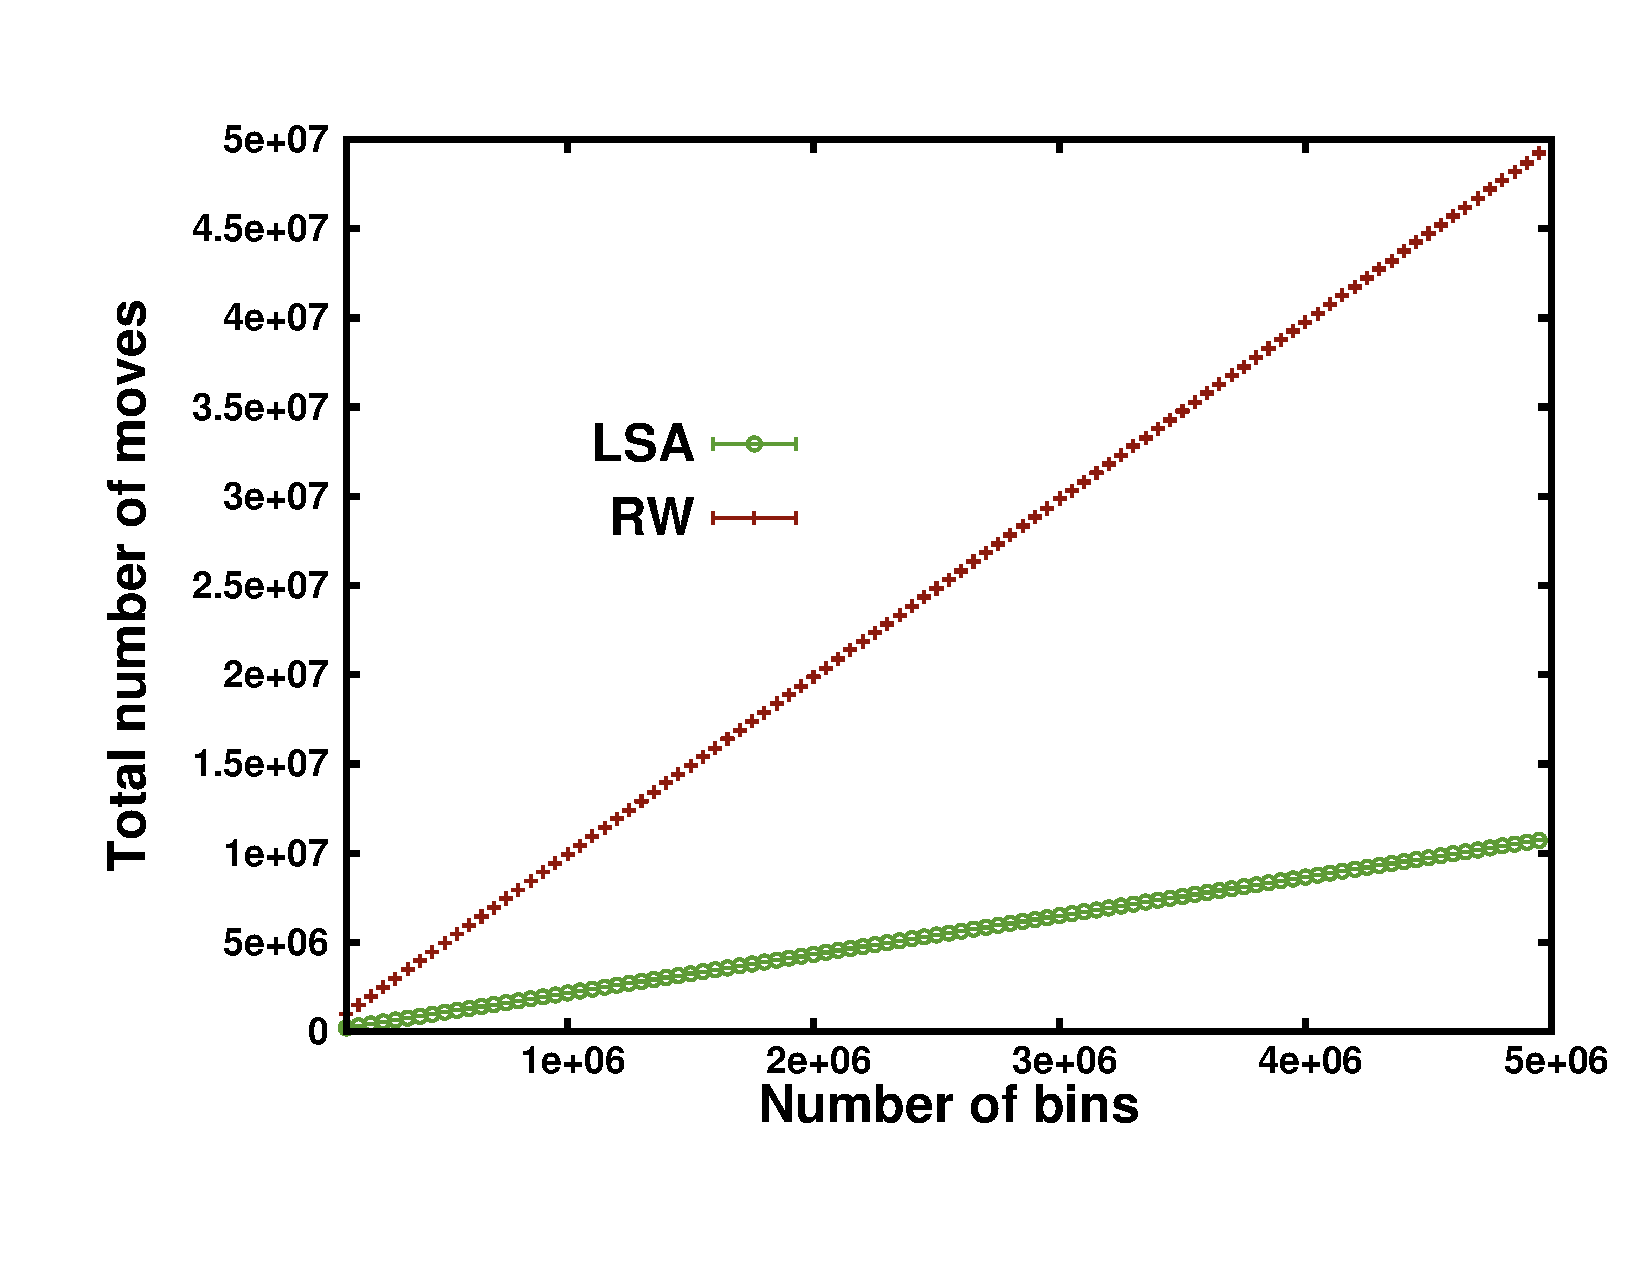
\includegraphics[width=0.45\textwidth]{total-3.pdf}}
   \quad
     \subfigure[$k=4$, $c=0.97 ~(c^*_4\approx 0.976)$] {\label{fig:all-3}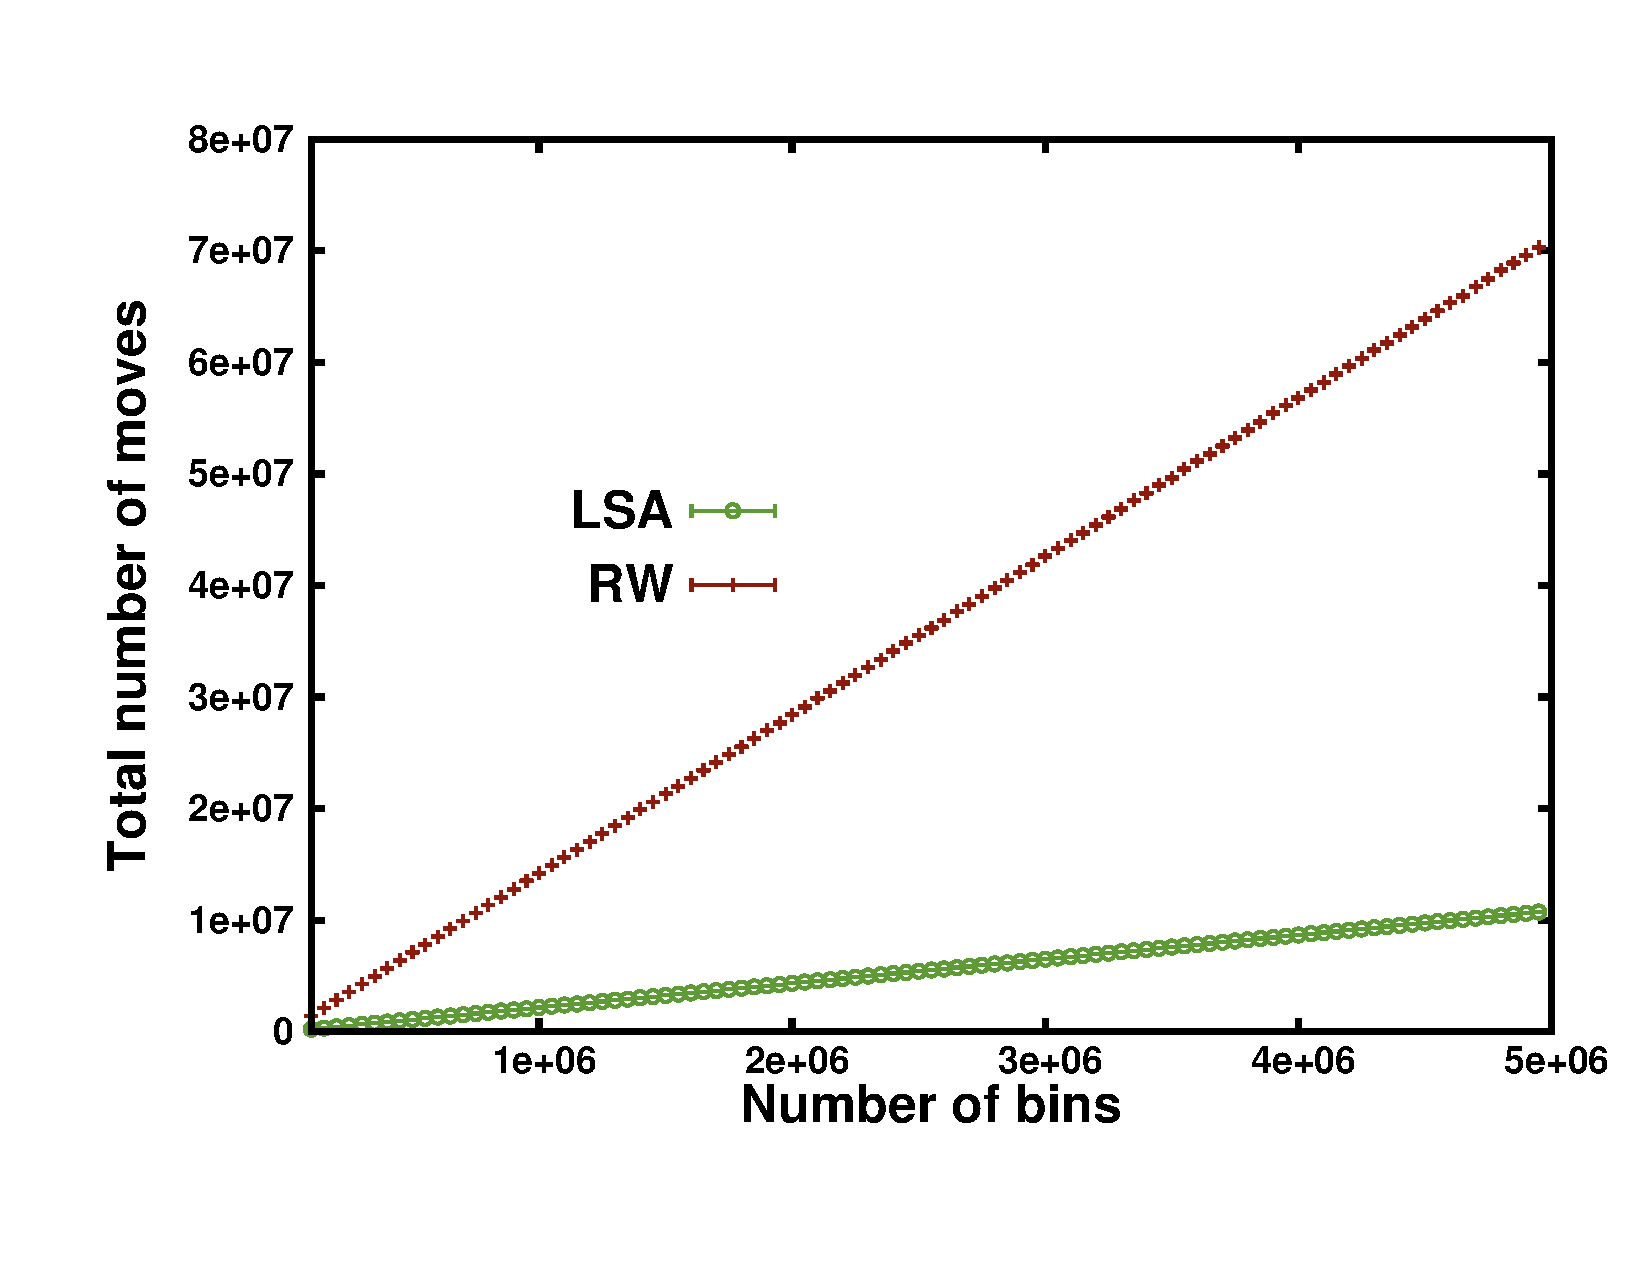
\includegraphics[width=0.45\textwidth]{total-4.pdf}}
     \vspace{-8pt}
   \caption{Comparison of total number of moves performed by local search and random walk methods.}
   \label{fig:1}
\end{figure*}
\begin{figure*}[h!]  
   \centering  
    \subfigure[ $k=3$, $c=0.90 ~(c^*_3\approx 0.917)$.]{\label{fig:max}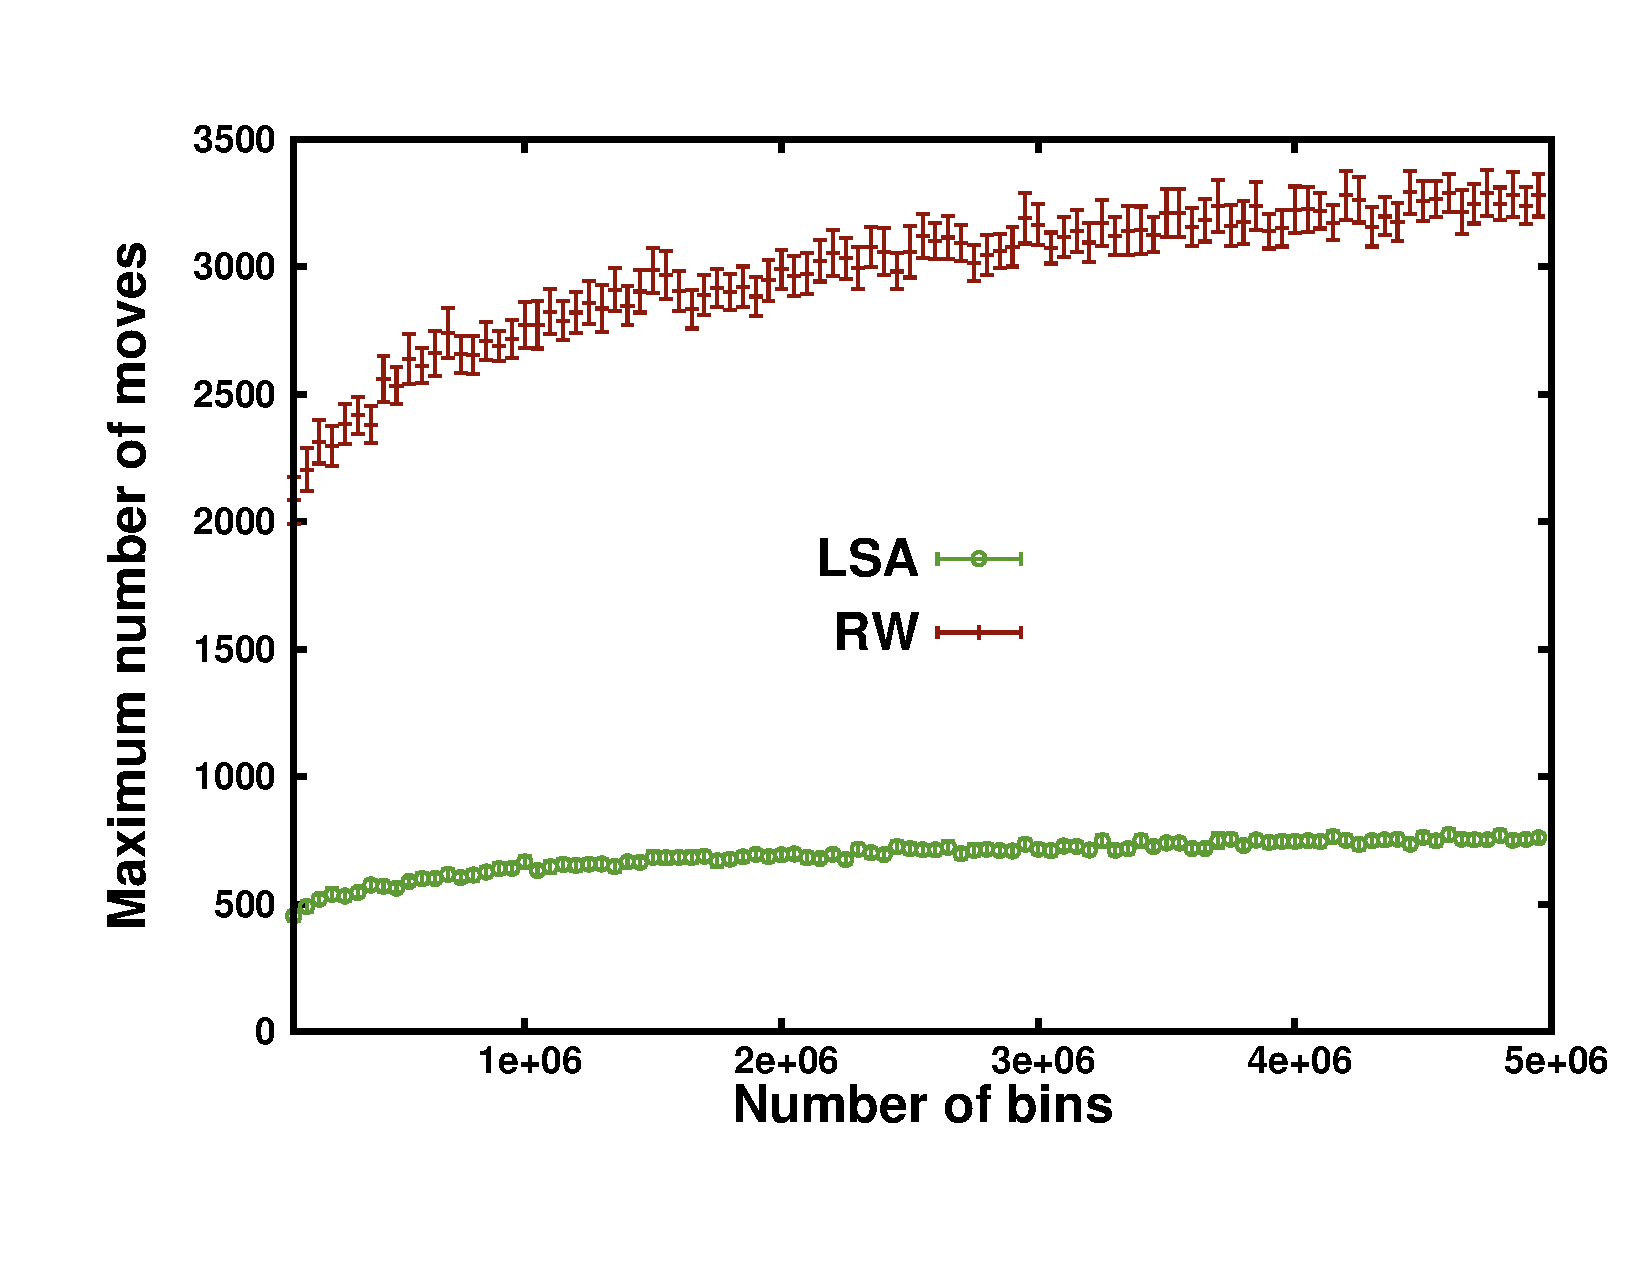
\includegraphics[width=0.45\textwidth]{max-3.pdf}}
   \quad
 \subfigure[$k=4$, $c=0.97 ~(c^*_4\approx 0.976)$.]{\label{fig:his to-3}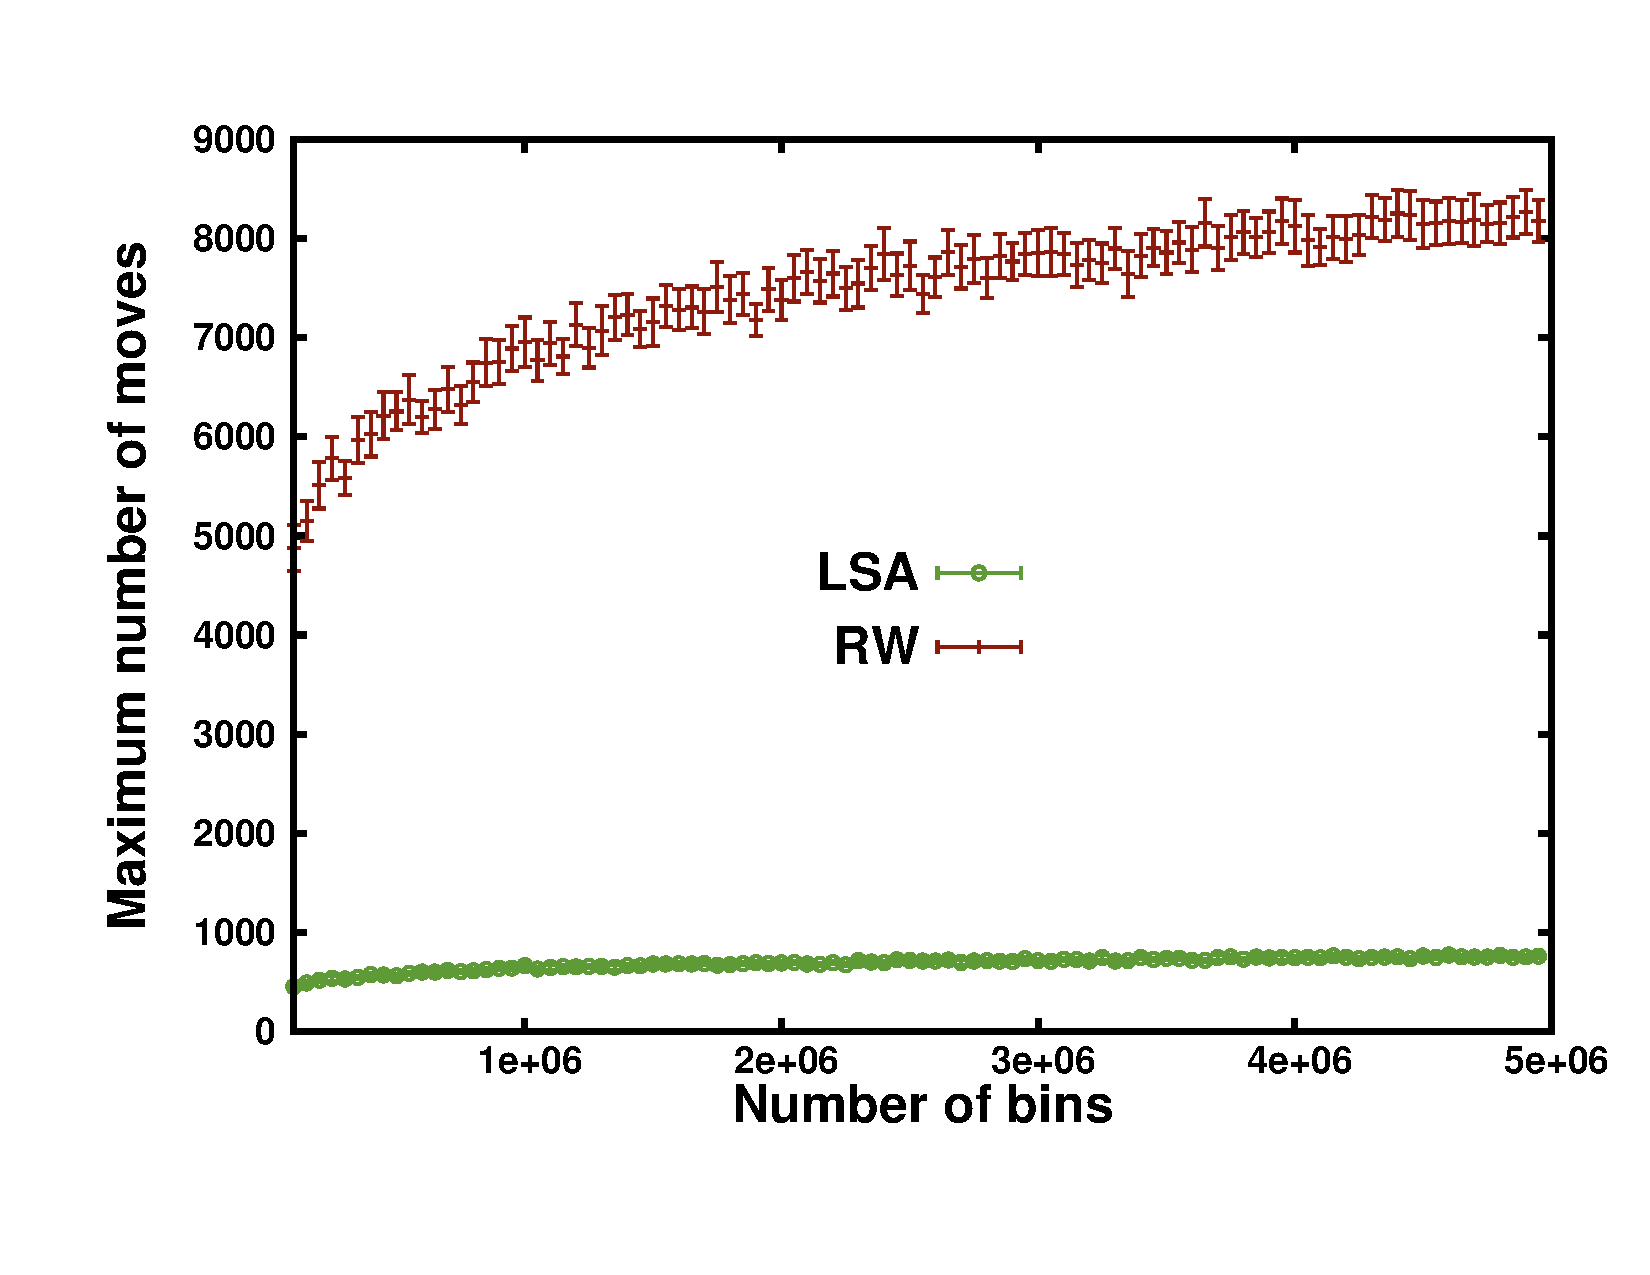
\includegraphics[width=0.45\textwidth]{max-4.pdf}}
   \vspace{-8pt}
   \caption{Comparison of maximum number of moves performed by local search and random walk methods}
    \label{fig:2}
\end{figure*}
\begin{figure*}[h!]
   \centering  
     \subfigure[$k=3$, $c\le 0.915 ~(c^*_3\approx 0.917)$]{\label{fig:fix-3}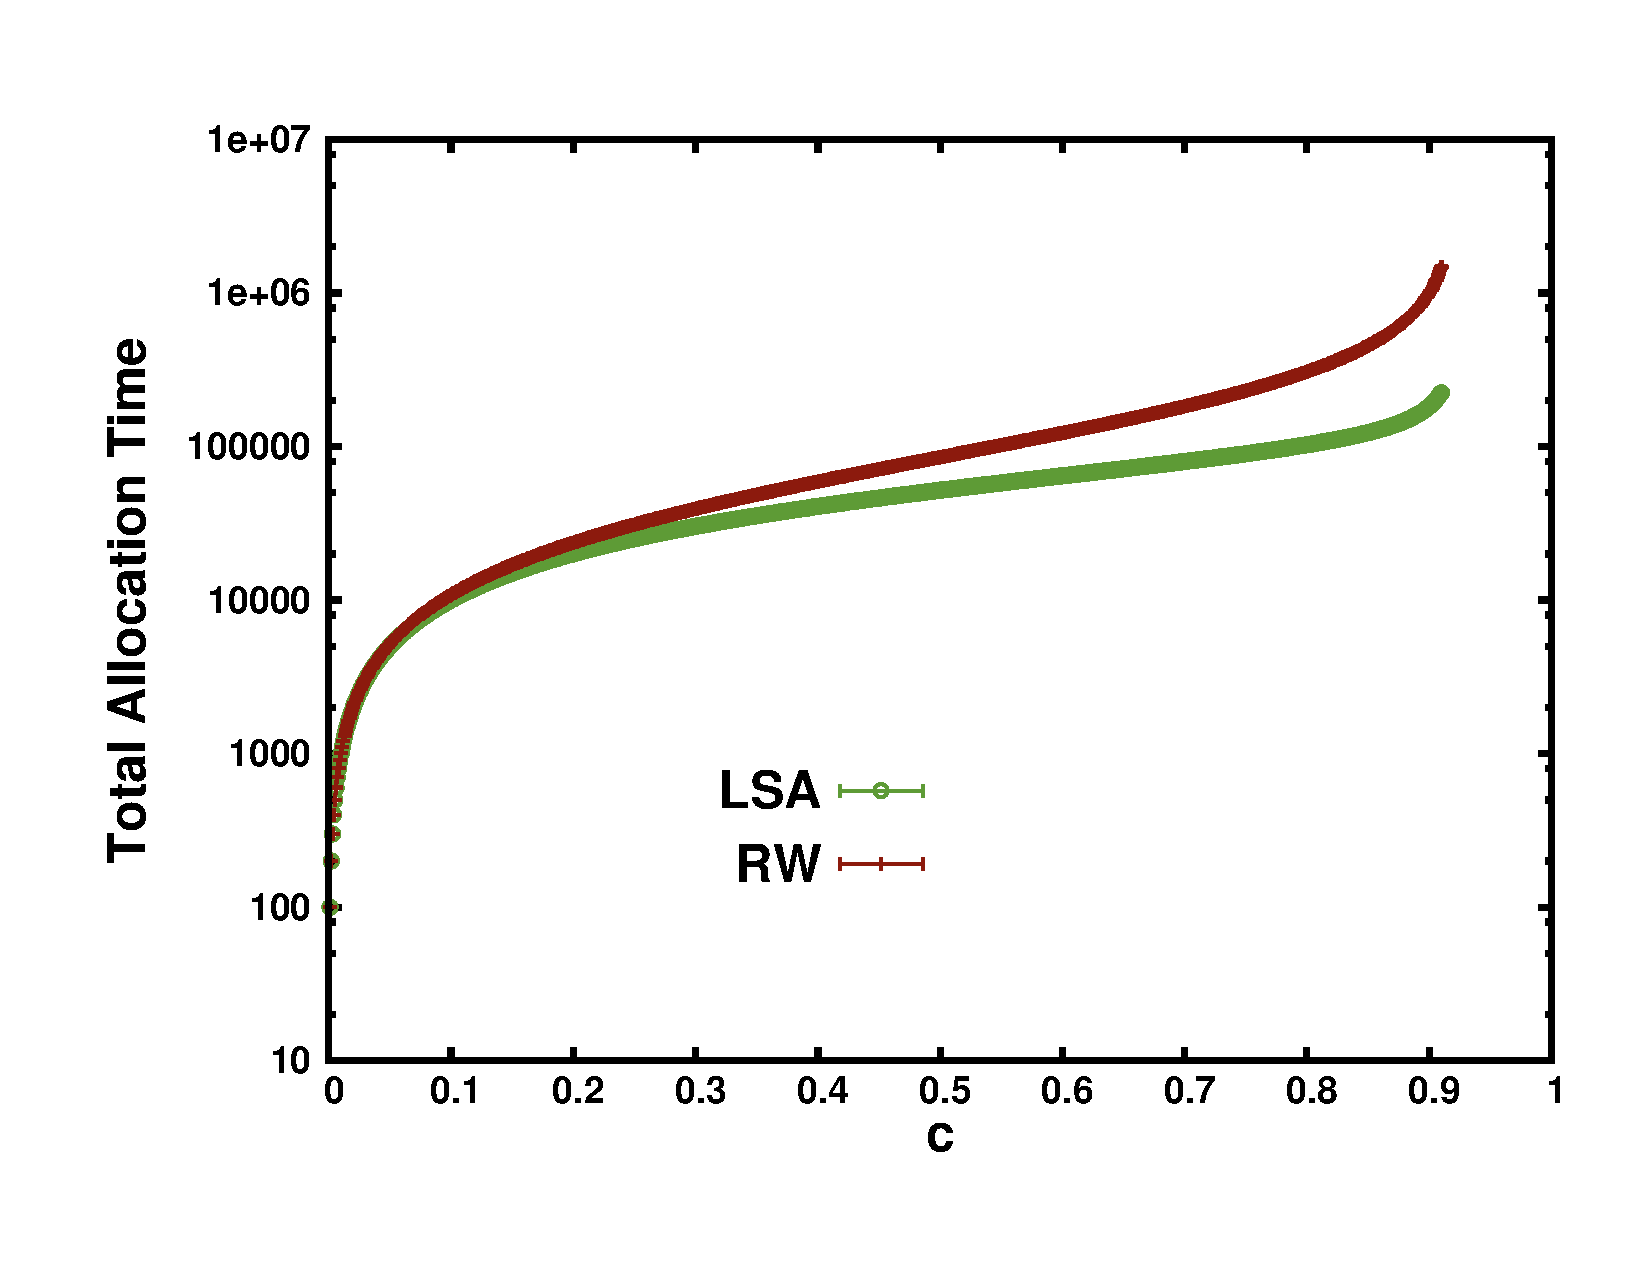
\includegraphics[width=0.45\textwidth]{totald-3.pdf}}
   \quad
       \subfigure[$k=3$, $c\le0.915 ~(c^*_3\approx 0.917)$] {\label{fig:fix-3-total}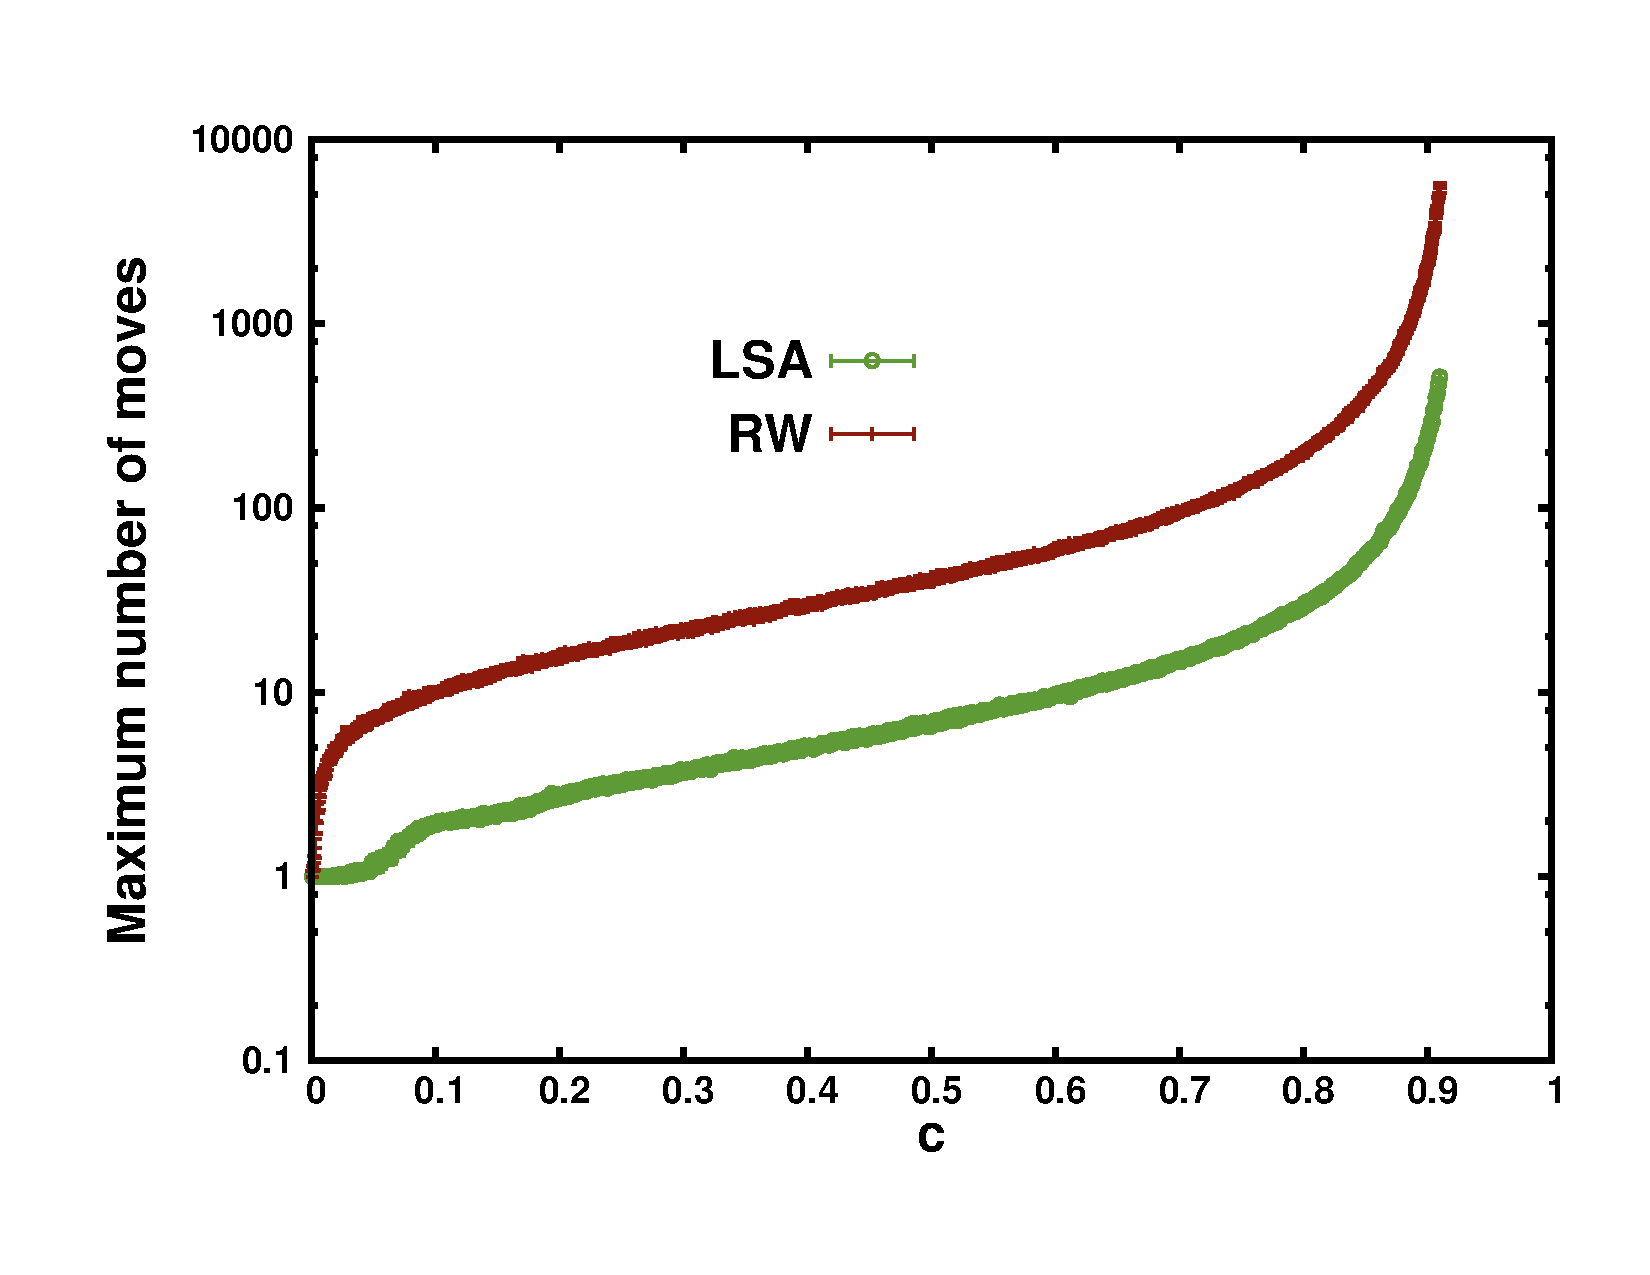
\includegraphics[width=0.45\textwidth]{maxd-3.pdf}}
       \vspace{-8pt}
   \caption{ Comparison of total number of moves and maximum number of moves (for fixed number of locations, $n=10^5$) performed by local search and random walk methods when density c approaches $c^*_k$.}
      \vspace{-1pt}
   \label{fig:3}
\end{figure*}
\begin{figure}[h!]
   \centering  
    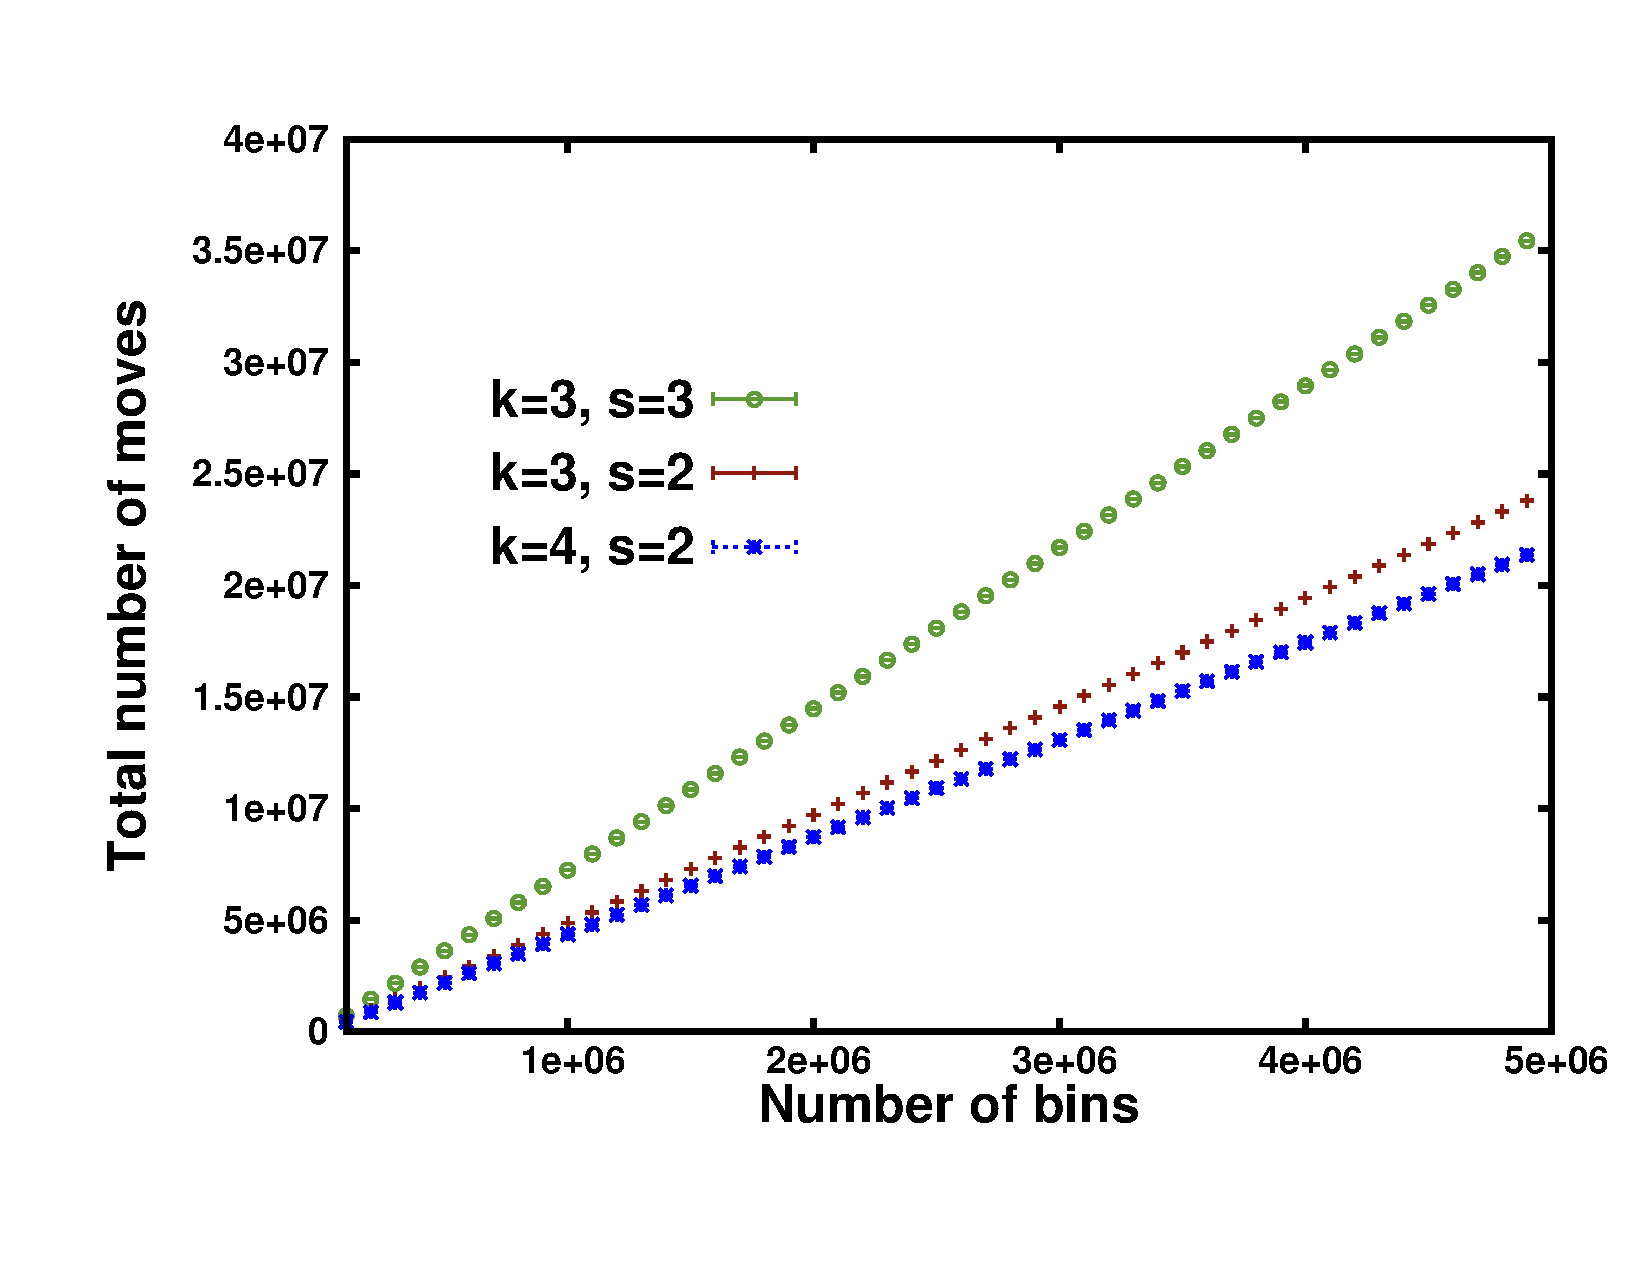
\includegraphics[width=0.85\textwidth]{totalGen-3-2.pdf}
    \caption{Total number of moves for the case where bin capacities (maximum load, $s$) is greater than 1.}
    \label{fig:totalGen}
    \end{figure}

We remark that local search allocation has some additional cost, i.e., the extra space required to store the labels. Though this space is $O(n)$, local search allocation is still useful for the applications where the size of objects (representing the balls) to be allocated is much larger than the labels which are integers. Moreover, with high probability, the maximum label of any vertex is $O(\log n)$. Many integer compression methods~\cite{inp:sgl10} have been proposed for compressing small integers and can be potentially useful in our setting for further optimizations. Also in most of the load balancing problems, the speed of finding an assignment is a much desired and the most important requirement.

We also consider the case when each bin can hold more than one ball. To adapt LSA for this setting we make a small change, i.e., the label of a vertex (bin) stays 0 until it is fully filled. Algorithm~\ref{algo:orientEdgegen} gives the modified procedure for the general bin capacities. Here {\sc{Balls}}$(v)$ gives the number of balls already placed in $v$. Let the bin capacity or maximum load allowed be $s$. Figure~\ref{fig:totalGen} suggests that the total number of moves are linear in the number of bins for the cases $k=3,4$ where the maximum bin capacity is greater than $1$.


\begin{table*}[ht!]
\centering
\footnotesize
\begin{tabular}{@{}l l l l @{}}
\toprule
%\hline \noalign{\smallskip}
\multicolumn{1}{l}{} & Limit on Moves                  & Wall-clock times     & Result Size  \\
\hline \noalign{\smallskip}
LSA        &   1      & 12    & 1029449  \\
       &   2      & 12    & 1080006  \\
        &   4      & 12    & 1082199  \\
        &   5      & 16    & 1082214  \\
        &   10      & 15    & 1082214  \\
        &   50     & 15    & 1082214  \\
        &   100     & 15    & 1082214  \\
        &   1000     & 15    & 1082214  \\
        &   10000    & 27    & 1082214  \\
        &   100000    & 136    & 1082214  \\
        &   $n$    & 1887    & 1082214  \\
\midrule

Hopcroft-Karp                &  & 12605 & 1082214 \\
%\hline \noalign{\smallskip}

\hline \noalign{\smallskip}
\end{tabular}
\caption{Performance of LSA on \textsf{Delicious} dataset. Time is measured in seconds.}
\label{table:softlabel}
\end{table*}

\subsection{Performance on Real-world graphs}

Next, we compare our runtime performance to the optimal algorithm proposed by Hopcroft et al.~\cite{hopcroft1973n}. In this experiment we want to study the effect of number of allowable moves on (a) the actual wall-clock times , (b) the result quality in terms of the size, or number of edges, of the final matching produced (refer Figure~\ref{table:softlabel}). We selected the following representative realworld datasets for our experiments:

\begin{itemize}
  \item \textsf{Delicious dataset : } The \textsf{Delicious} dataset spans nine years from 2003 to 2011 and contain about 340 mio. bookmarks, 119 mio. unique URLs, 15 mio. tags and 2 mio. users~\cite{zubiaga2013harnessing}. Each bookmarked URL is time stamped and tagged with word descriptors. The nodes in one of the sets are URLs and in the other are its corresponding bookmarks.

  \item \textsf{Yahoo Ad dataset : } Computational advertising used bi-partite graph matching algorithms for its ad placement decisions. 
\end{itemize}

We first observe that the optimal result in the \textsf{Delicious} dataset, i.e. 1082214, is already obtained when the limit on the allowable moves is only five and in 12 seconds. Interestingly, as we increase the limit on the allowable moves, the runtime does not change showing that only a small of defections are sufficient to arrive at an optimal result. However, at higher limits, indeed other permutations are explored (in this case unsuccesfully) resulting in increased runtimes. In any case when the limit is set to $n$, that would guarantee optimality, we still perform an order of magnitude faster than the optimal algorithm of Hopcroft-Karp. 








%\begin{proposition}\label{prop:levelSize}
%For any orientation $O$ of $H_{n,m,k}$, let R be the set of farthest vertices from F. For each $i\le \Delta$ the number of vertices at distance $\Delta-i$ from $F$ is atmost ${|R|\cdot (k-1)}^{i}$.
%\end{proposition}
%We now have the following corollary.
%\begin{corollary}\label{cor:sum}
%Let $h$ be any orientation of a random hypergraph $H_{n,m,k}$ and $L(i)$ be the level of vertex $i$ w.r.t. orientation $h$. Then $\sum_i L(i) = O(n)$ w.h.p. 
%\end{corollary}
%\begin{proof}
%
%From Proposition~\ref{prop:lev} we know that for any vertex $i$, the level $L(i)$ is at most the distance from a free vertex.  By Lemma~\ref{lem:dist} we know that with high probability, there is a linear fraction of vertices which are at a constant distance from the set of free vertices. Let $S$ denote the set of these vertices. Hence, with high probability the following holds. In particular, everything we state about the distances of vertices from $F$ holds with high probability.
%\[
%\sum_i L(i) \le \sum_{i  \notin S} L(i) + O(n).
%\]
%Let $T(i)$ denotes the true distance of a vertex $v$ from some free vertex in the orientation graph. Then
%\[ \sum_{i  \notin S} L(i) \le \sum_{i  \notin S} T(i). \]
%Let us denote the number of vertices in a level $\ell$ by $N_{\ell}$. By Proposition~\ref{prop:levelSize} we have 
%  $N_{\ell} \le {|R|\cdot (k-1)}^{i}$, where $R$ is the set of vertices at the deepest level. Thus we can obtain an estimate of the number of vertices in the set $V \setminus S \cup F$ by the following.
%  \[   \mathcal{W}= \sum_{\ell = 0}^{\Delta-1} |R|\cdot (k-1)^{\ell} .\]
%  Thus, we over count the number of vertices in the concerned set by at least $n- \mathcal{W}$. 
%  Now,
%  \[\sum_{i  \notin S} T(i)= \sum_{j=0}^{\Delta-1} (\Delta-j) {N_j}.\]
%  
%Substituting $N_j \le{ (k-1)}^{j}$, we over count the above sum at least $n- \mathcal{W}$. This is true because the contribution made by each of these dummy vertices (in the level counting sum) is at least $1$. Therefore, 
%  \begin{align} 
%\begin{split}
%\sum_{i  \notin S} T(i) \le & \sum_{j=0}^{\Delta-1} (\Delta-j) {|R|\cdot (k-1)}^{j}- (n-\mathcal{W})\\
%=& \Delta |R|\cdot \sum_{j=0}^{\Delta-1}{(k-1)}^j - |R|\cdot \sum_{j=0}^{\Delta-1} j{(k-1)}^j - (n-\mathcal{W})\\
%=& \Delta |R|\cdot \left({{(k-1)}^{\Delta}-1 \over k-2 } -\Delta {{(k-1)}^{\Delta} \over k-2}\right) + \sum_{\ell = 0}^{\Delta-1} |R|\cdot (k-1)^{\ell}- (n-\mathcal{W})\\
%=&O(n).
%\end{split}
%\end{align}
%\end{proof}
%\begin{proof}[Proof of Theorem~\ref{thm:main}]
%The proof of our main theorem follows from Lemma~\ref{lem:graph} and Corollary~\ref{cor:sum}.
%\end{proof}


%\section{Experimental Evaluation of Random and Quasi Random Orientation}\label{sec:exp}
%In order to draw comparisons between variants of orientation procedure, we present some experiments. We also demonstarte the potential importance of our new algorithm in practical settings.
%
%We consider a random hypergraph with $n=10000$ vertices and insert upto $(c^*_k-0.01)n$ edges each having $k$ random choices. We cosider random walk, quasi random and level walks for orientation. We average the total insertion time over 30 iterations for each of these methods. The following plot for $k=3$ draws a clear comparison in the performance of these variants.
%\begin{figure}[h!]
%\begin{centering}
% \includegraphics[scale=0.75]{totalComp.pdf}
%	 \end{centering}
%	 \caption{ For $k=3$, with $10000$ vertices and upto $9000$ edges}
%\end{figure}
%We also average the maximum insertion time over 30 iterations for each of these methods. The log plot is shown in Figure~\ref{fig:maxIns}.
%\begin{figure}[h!]\label{fig:maxIns}
% \includegraphics[scale=1]{comp.pdf}
%	 \caption{ For $k=3$, with $10000$ vertices and upto $9000$ edges}
%\end{figure}
%\small
\bibliographystyle{plain}
\bibliography{FinalCuckooIns}
\end{document}
